\documentclass[../Carre_nights.tex]{subfiles}

\begin{document}

\section{n0905}
\textbf{\Large{The splendid tale of prince Diamond}} \\

\begin{figure}[ht]
\centering
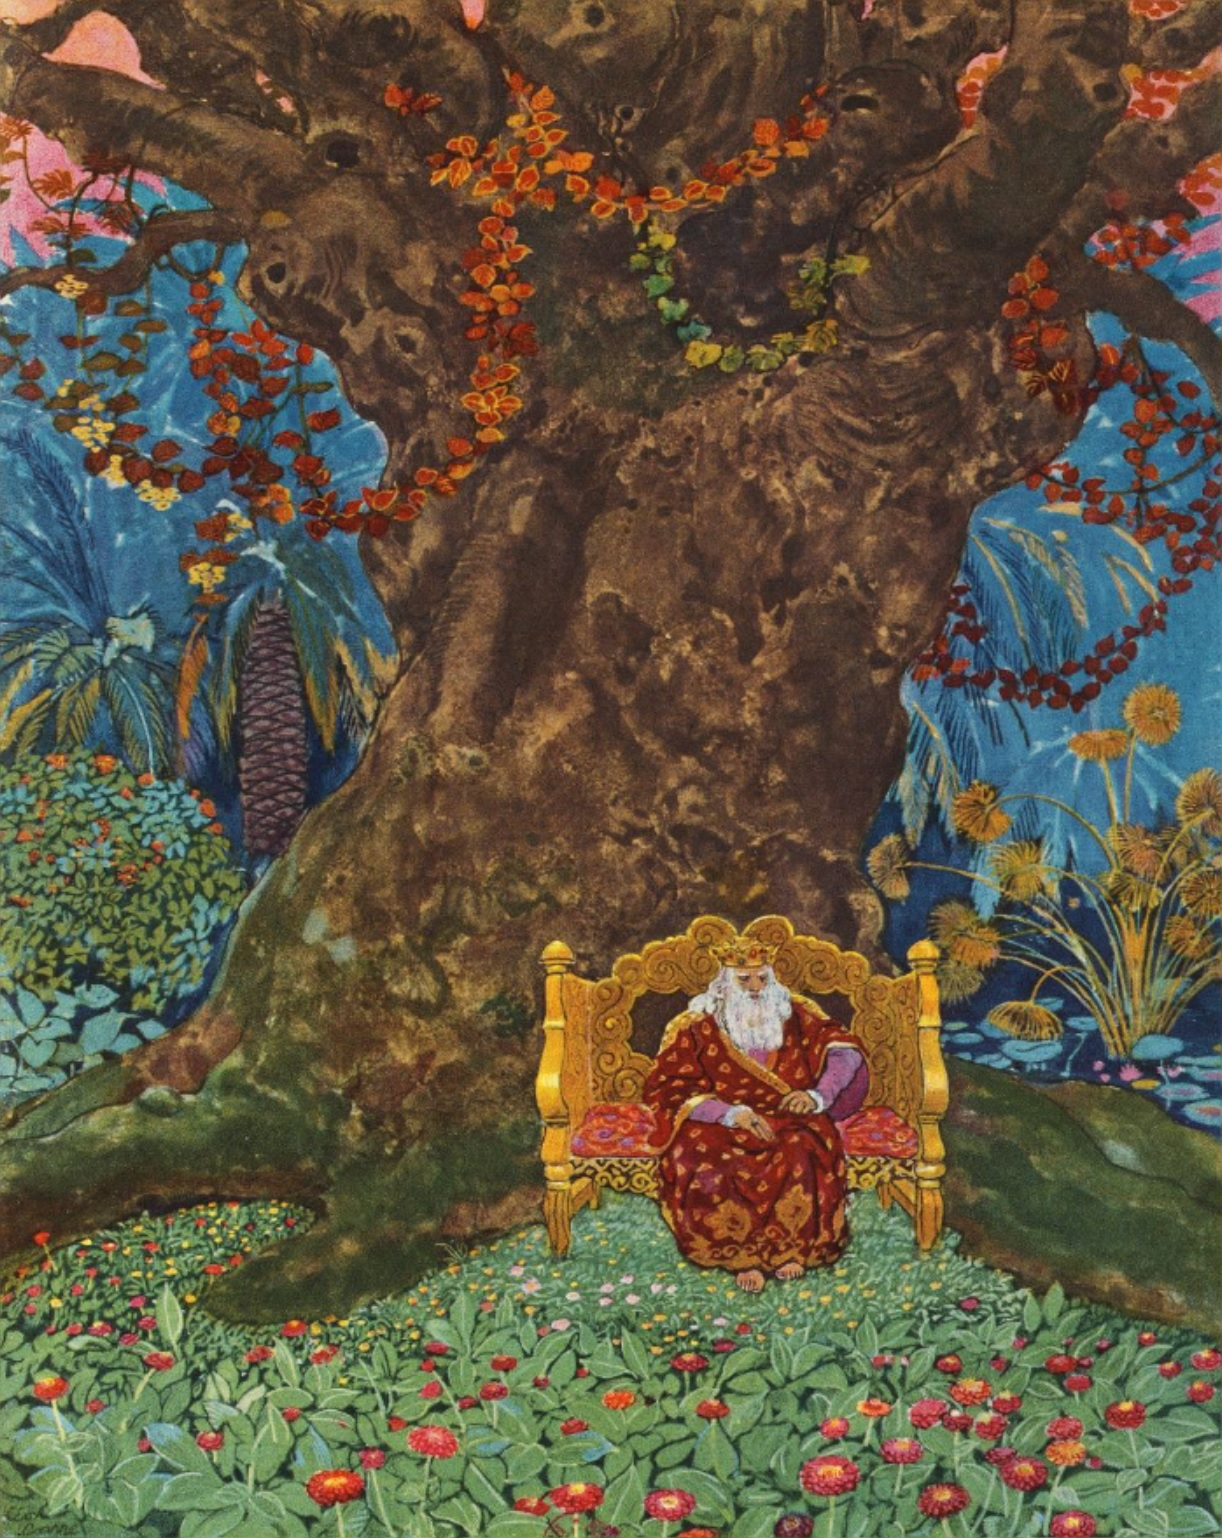
\includegraphics[height=\figsize]{illustrations/volume_8/T08, n0905 - Histoire splendide du prince Diamant.jpg}
\end{figure}

\textit{\\
"...voici qu’à l’abri d’un très vieil arbre, dont les racines devaient plonger jusqu’aux portes intérieures de la terre, il vit un trône solitaire. Et sur ce trône était assis un vieux roi, la tête couronnée de la couronne royale et les pieds nus, qui réfléchissait."} \\
—T08, n0905 - Histoire splendide du prince Diamant \\~\\
\textit{"...he noticed a lonely throne shaded by a very old tree whose roots must have reached to the innermost doors of earth. Upon this throne sat an aged King with a crown upon his head, and naked feet, who looked before him, wrapped in contemplation."} \\
—V04, n0905 - The splendid tale of prince Diamond

\newpage

\section{n0908}
\textbf{\Large{The splendid tale of prince Diamond}} \\

\begin{figure}[ht]
\centering
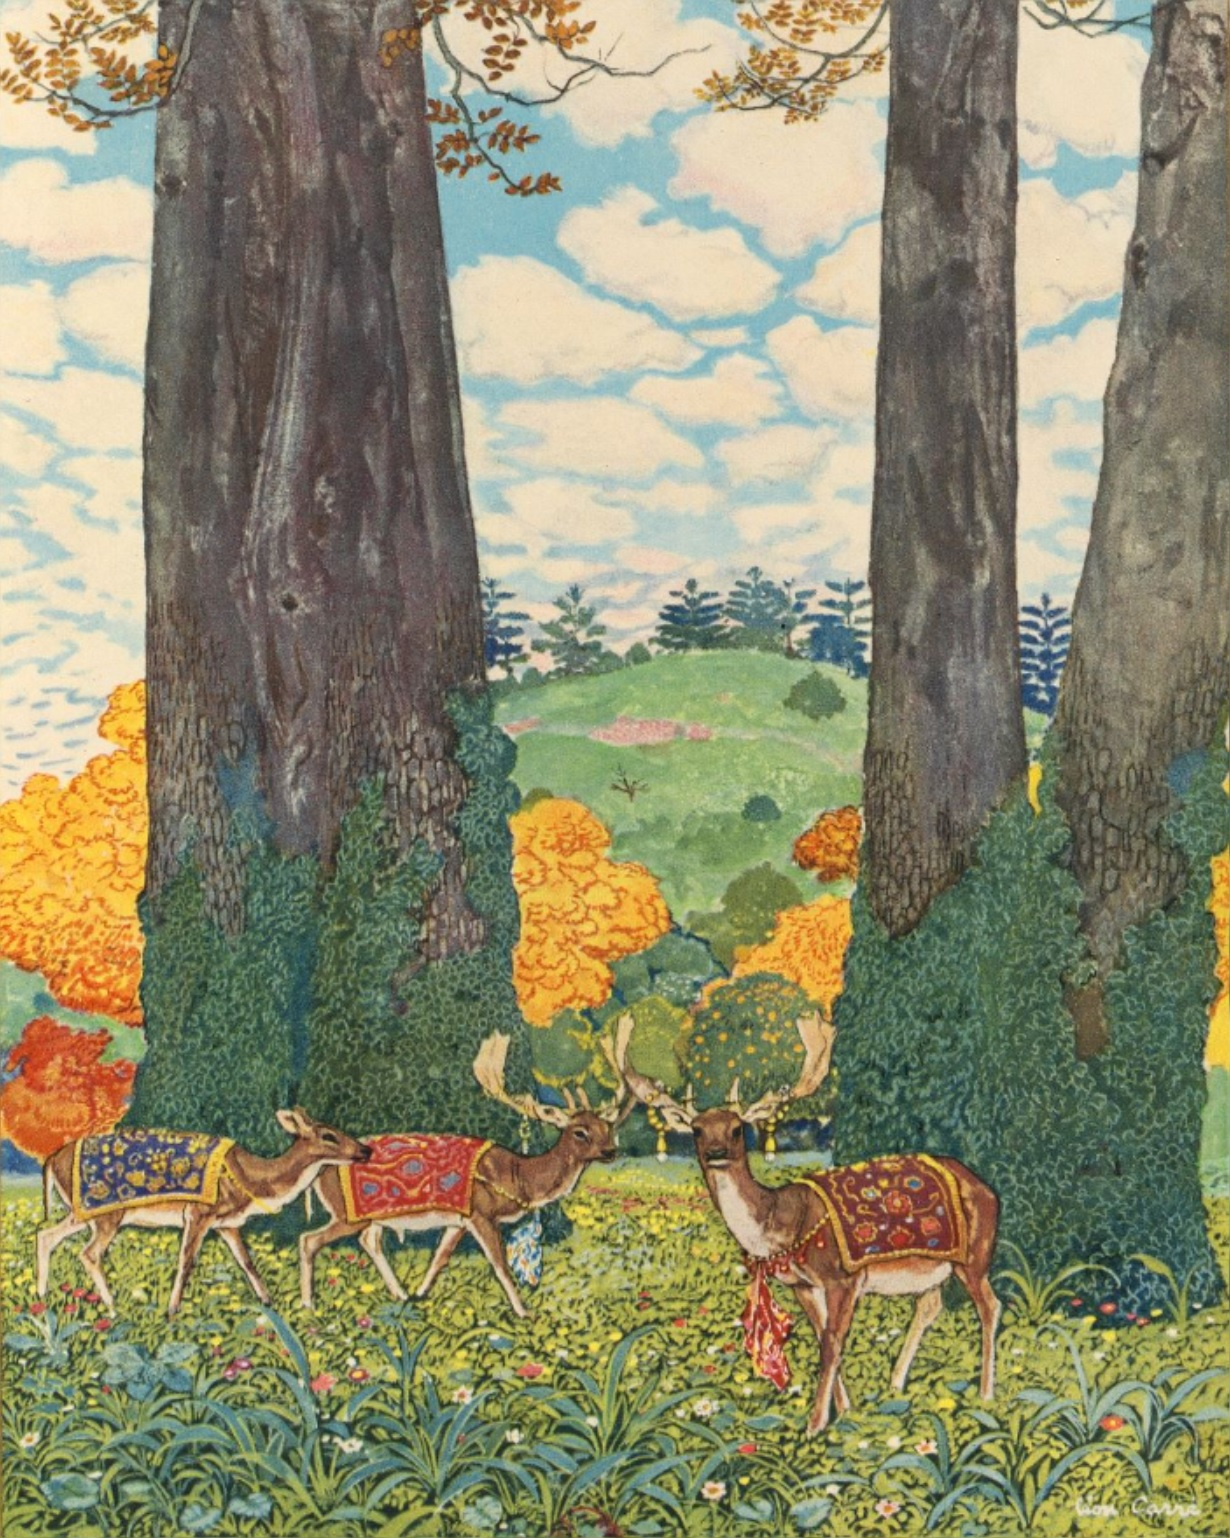
\includegraphics[height=\figsize]{illustrations/volume_8/T08, n0908 - Histoire splendide du prince Diamant.jpg}
\end{figure}

\textit{\\
"...l’air de ce jardin était si excellent que les branches des arbres se balançaient comme des gens ivres. Et au-dessous des arbres paissaient de grands daims, qui portaient, attachés à leurs cornes, des ornements d’or garnis de pierreries..."} \\
—T08, n0908 - Histoire splendide du prince Diamant \\~\\
\textit{"The air of the place was such that the trees wavered and balanced as if they had drunken wine; in and out among them walked great deer with ornaments of jewelled gold hung about their horns..."} \\
—V04, n0908 - The splendid tale of prince Diamond

\newpage

\section{n0924}
\textbf{\Large{Some jests and suggestions of the master of shifts and laughter}} \\

\begin{figure}[ht]
\centering
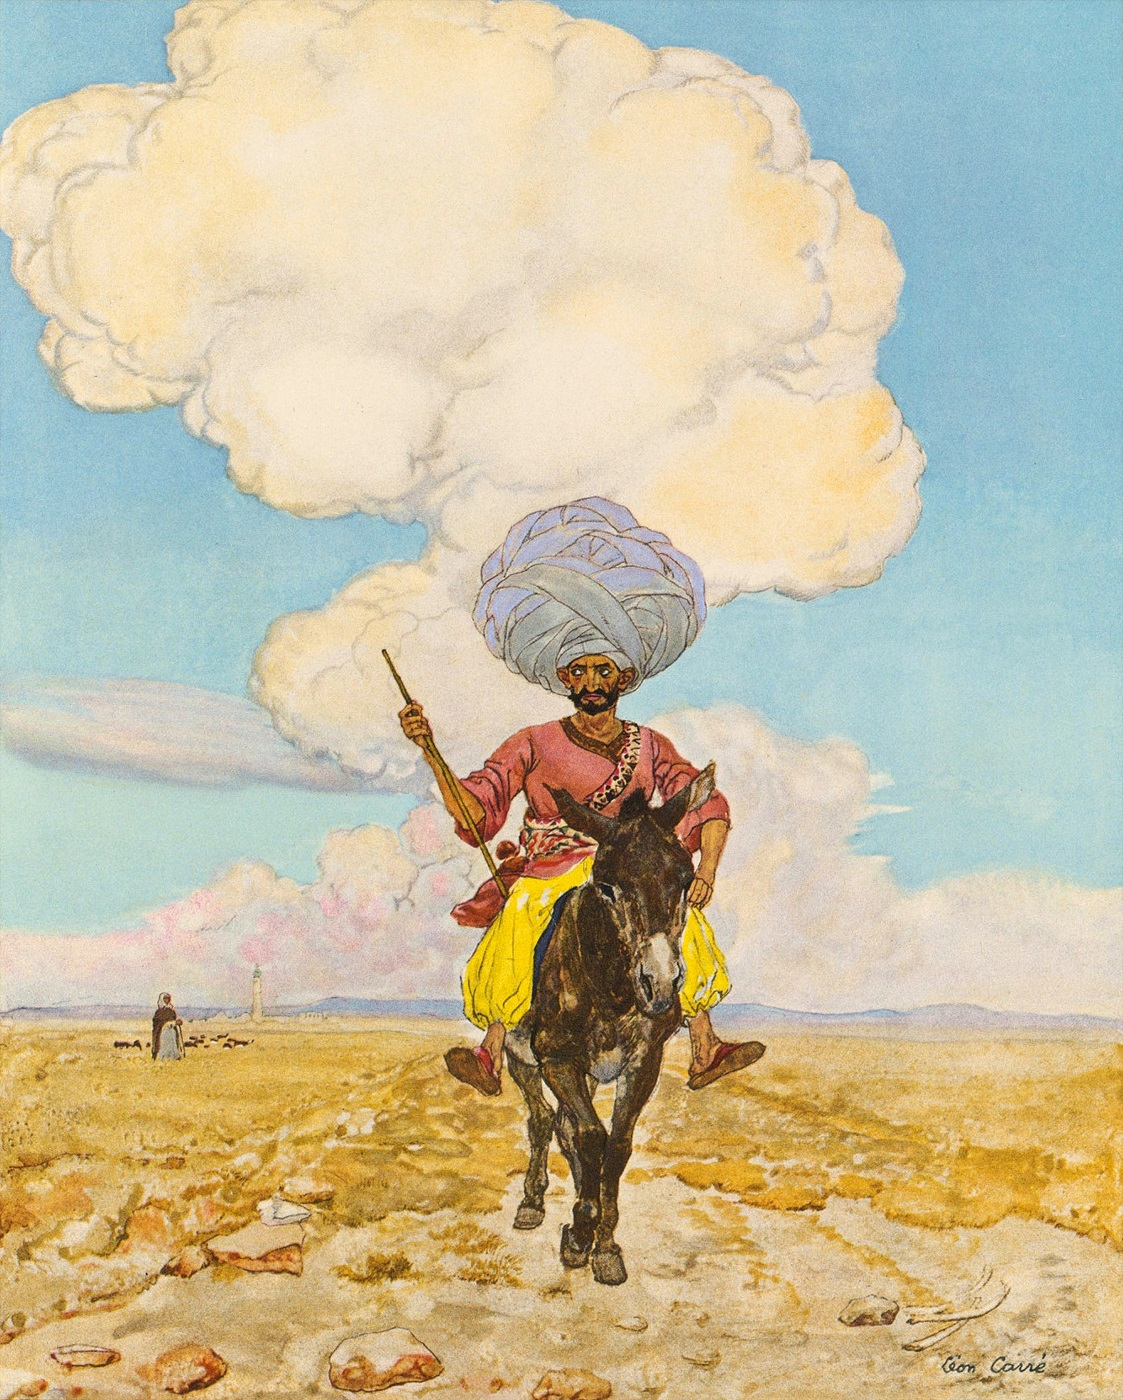
\includegraphics[height=\figsize]{illustrations/volume_8/T08, n0924 - Quelques sottises et théories du maître des devises et des ris.jpg}
\end{figure}

\textit{\\
"...Si-Goha fit apporter toute la mousseline disponible dans les souks, et s’en fabriqua un turban de la grandeur d’une roue de char. Puis il monta sur son âne..."} \\
—T08, n0924 - Quelques sottises et théories du maître des devises et des ris \\~\\
\textit{"He sent at once for all the muslin in all the shops of that place and rolled a turban as great as a chariot wheel about his head. Then he mounted his ass..."} \\
—V04, n0924 - Some jests and suggestions of the master of shifts and laughter

\newpage

\section{n0930}
\textbf{\Large{The tale of the girl Heart’s-Miracle}} \\

\begin{figure}[ht]
\centering
\includegraphics[height=\figsize]{illustrations/volume_8/T08, n0930 - Histoire de la jouvencelle Chef-d’oeuvre-des-Coeurs.jpg}
\end{figure}

\textit{\\
"...elle se vit dans une vaste prairie, si pleine de fleurs et de fraîcheur qu’on croyait voir une robe légère peinte de belles couleurs. Et au milieu de cette prairie s’élevait un palais..."} \\
—T08, n0930 - Histoire de la jouvencelle Chef-d’oeuvre-des-Coeurs \\~\\
\textit{"...she saw that they were traversing a vast meadowland, so filled with flowers that it appeared like a garment of painted silk below them. In the middle of this meadowland rose a palace..."} \\
—V04, n0930 - The tale of the girl Heart’s-Miracle

\newpage

\section{n0936}
\textbf{\Large{The tale of the girl Heart’s-Miracle}} \\

\begin{figure}[ht]
\centering
\includegraphics[height=\figsize]{illustrations/volume_8/T08, n0936 - Histoire de la jouvencelle Chef-d’oeuvre-des-Coeurs.jpg}
\end{figure}

\textit{\\
"...au bout d’un moment, il prit du cœur, et, appuyant sur la porte qui céda, il entra disant : « Bismillah ! Confondu soit le Malin ! Je me réfugie en Allah contre les maléfices ! »"} \\
—T08, n0936 - Histoire de la jouvencelle Chef-d’oeuvre-des-Coeurs \\~\\
\textit{"Al-Rashid heard the singing and playing of his mistress; for a full minute he fumbled with the key in the lock, and then hurled himself into the room, calling to Allah against the wiles of the Devil."} \\
—V04, n0936 - The tale of the girl Heart’s-Miracle

\newpage

\section{n0938}
\textbf{\Large{The tale of Al-Malik Baibars [The first captain’s tale]}} \\

\begin{figure}[ht]
\centering
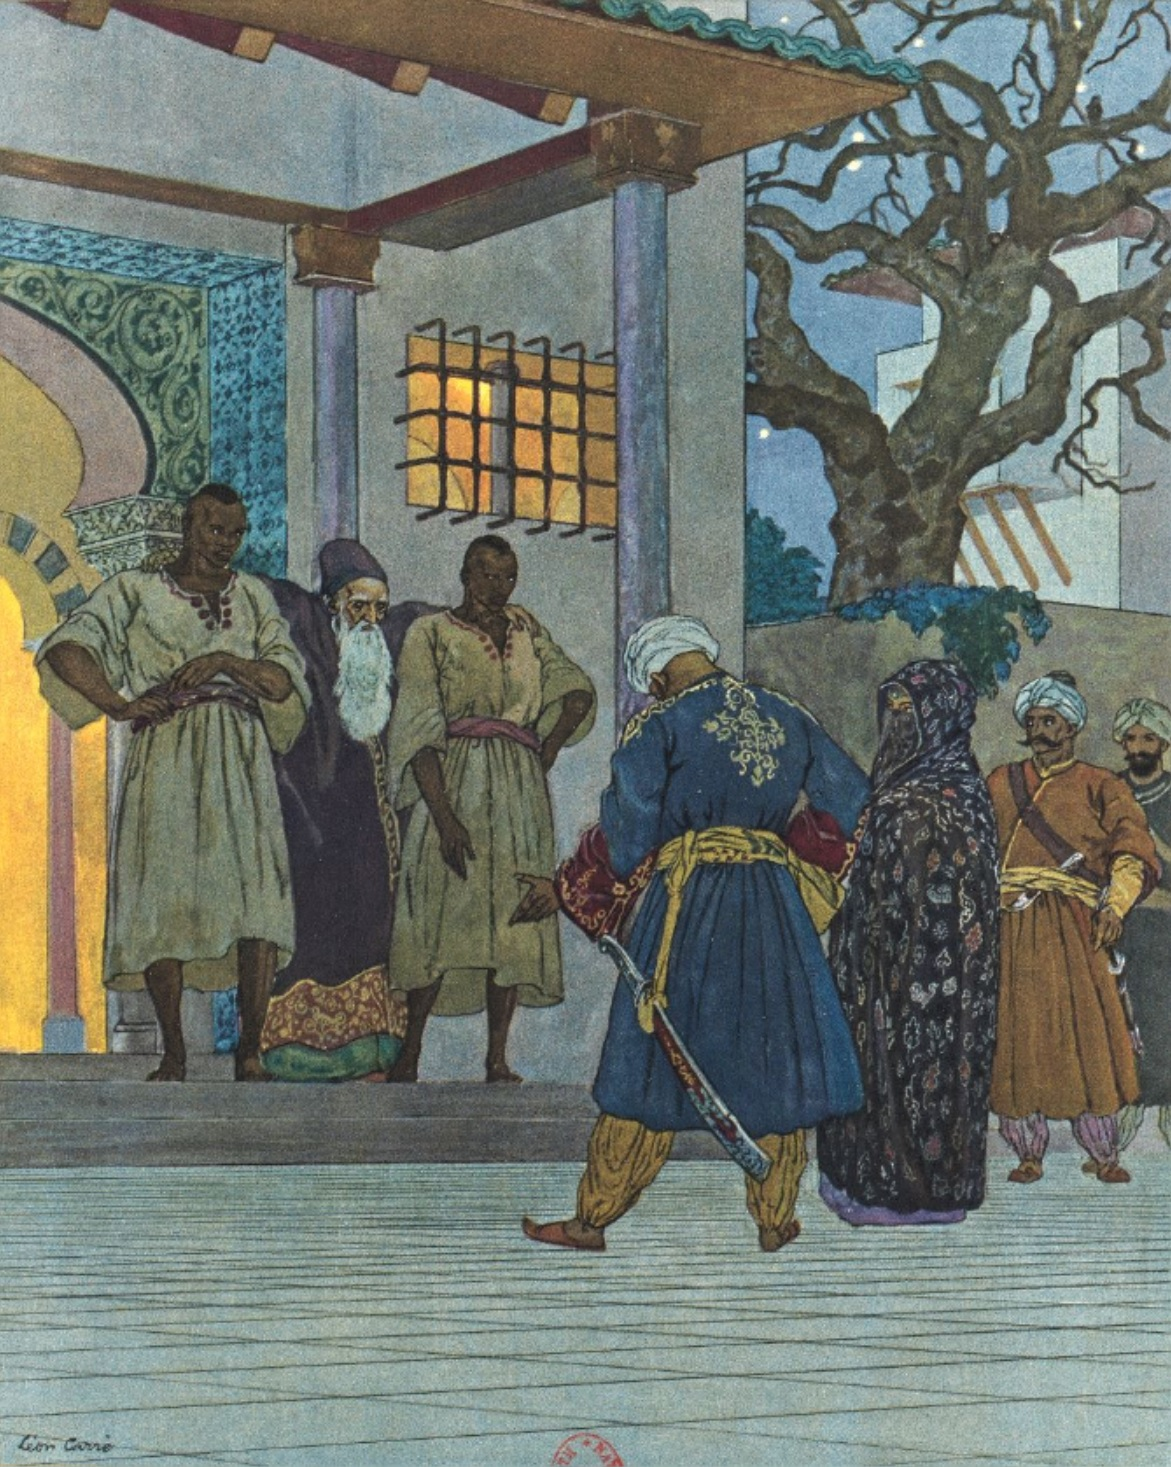
\includegraphics[height=\figsize]{illustrations/volume_8/T08, n0938 - Histoire de Baïbars [Histoire racontée par le premier capitaine].jpg}
\end{figure}

\textit{\\
"...le kâdi lui-même, appuyé sur les épaules de deux esclaves nègres, apparut à l’entrée. Et, après les salams de part et d’autre, je lui racontai l’affaire et lui soumis le cas, tandis que l’adolescente se tenait debout, soigneusement enveloppée de ses voiles."} \\
—T08, n0938 - Histoire de Baïbars [Histoire racontée par le premier capitaine] \\~\\
\textit{"...the judge appeared in person, leaning upon the shoulders of two black slaves. After greeting, I explained the affair to the old man, while the girl stood meekly to one side, with her veils drawn close about her."} \\
—V04, n0938 - The tale of Al-Malik Baibars [The first captain’s tale]

\newpage

\section{n0941}
\textbf{\Large{The tale of Al-Malik Baibars [The third captain’s tale]}} \\

\begin{figure}[ht]
\centering
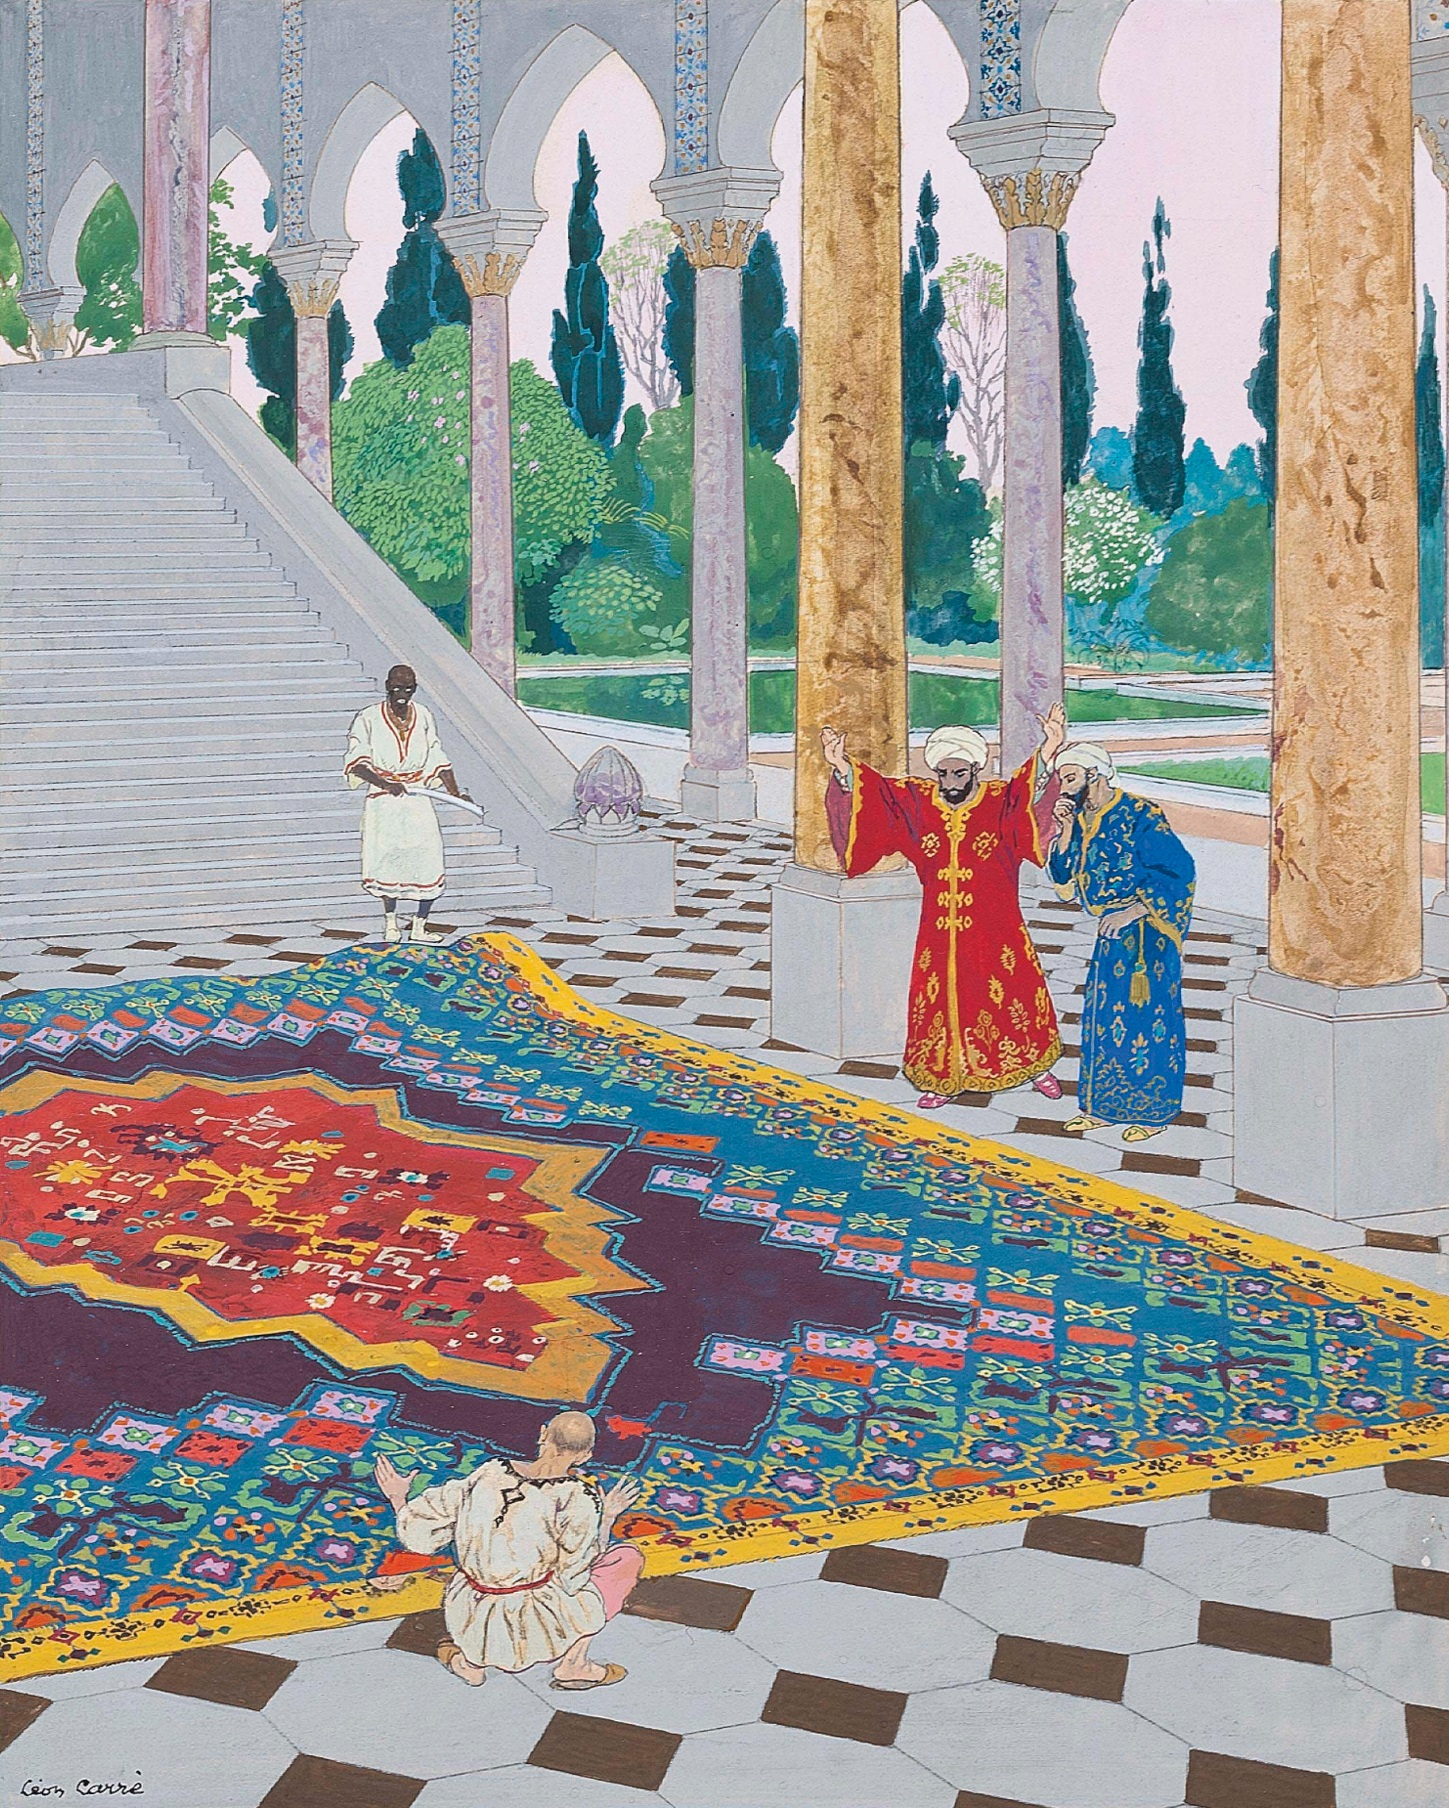
\includegraphics[height=\figsize]{illustrations/volume_8/T08, n0941 - Histoire de Baïbars [Histoire racontée par le troisième capitaine].jpg}
\end{figure}

\textit{\\
"...voici qu’un tapis magnifique s’étendit et se développa le long de la salle, dans tous les sens, dont il ne se trouvait pas le pareil dans le palais."} \\
—T08, n0941 - Histoire de Baïbars [Histoire racontée par le troisième capitaine] \\~\\
\textit{"...lo! a magnificent carpet began to stretch out from the nail and had soon covered the whole space of the floor with a fabric of unequalled beauty."} \\
—V04, n0941 - The tale of Al-Malik Baibars [The third captain’s tale]

\newpage

\section{n0942}
\textbf{\Large{The tale of Al-Malik Baibars [The fourth captain’s tale]}} \\

\begin{figure}[ht]
\centering
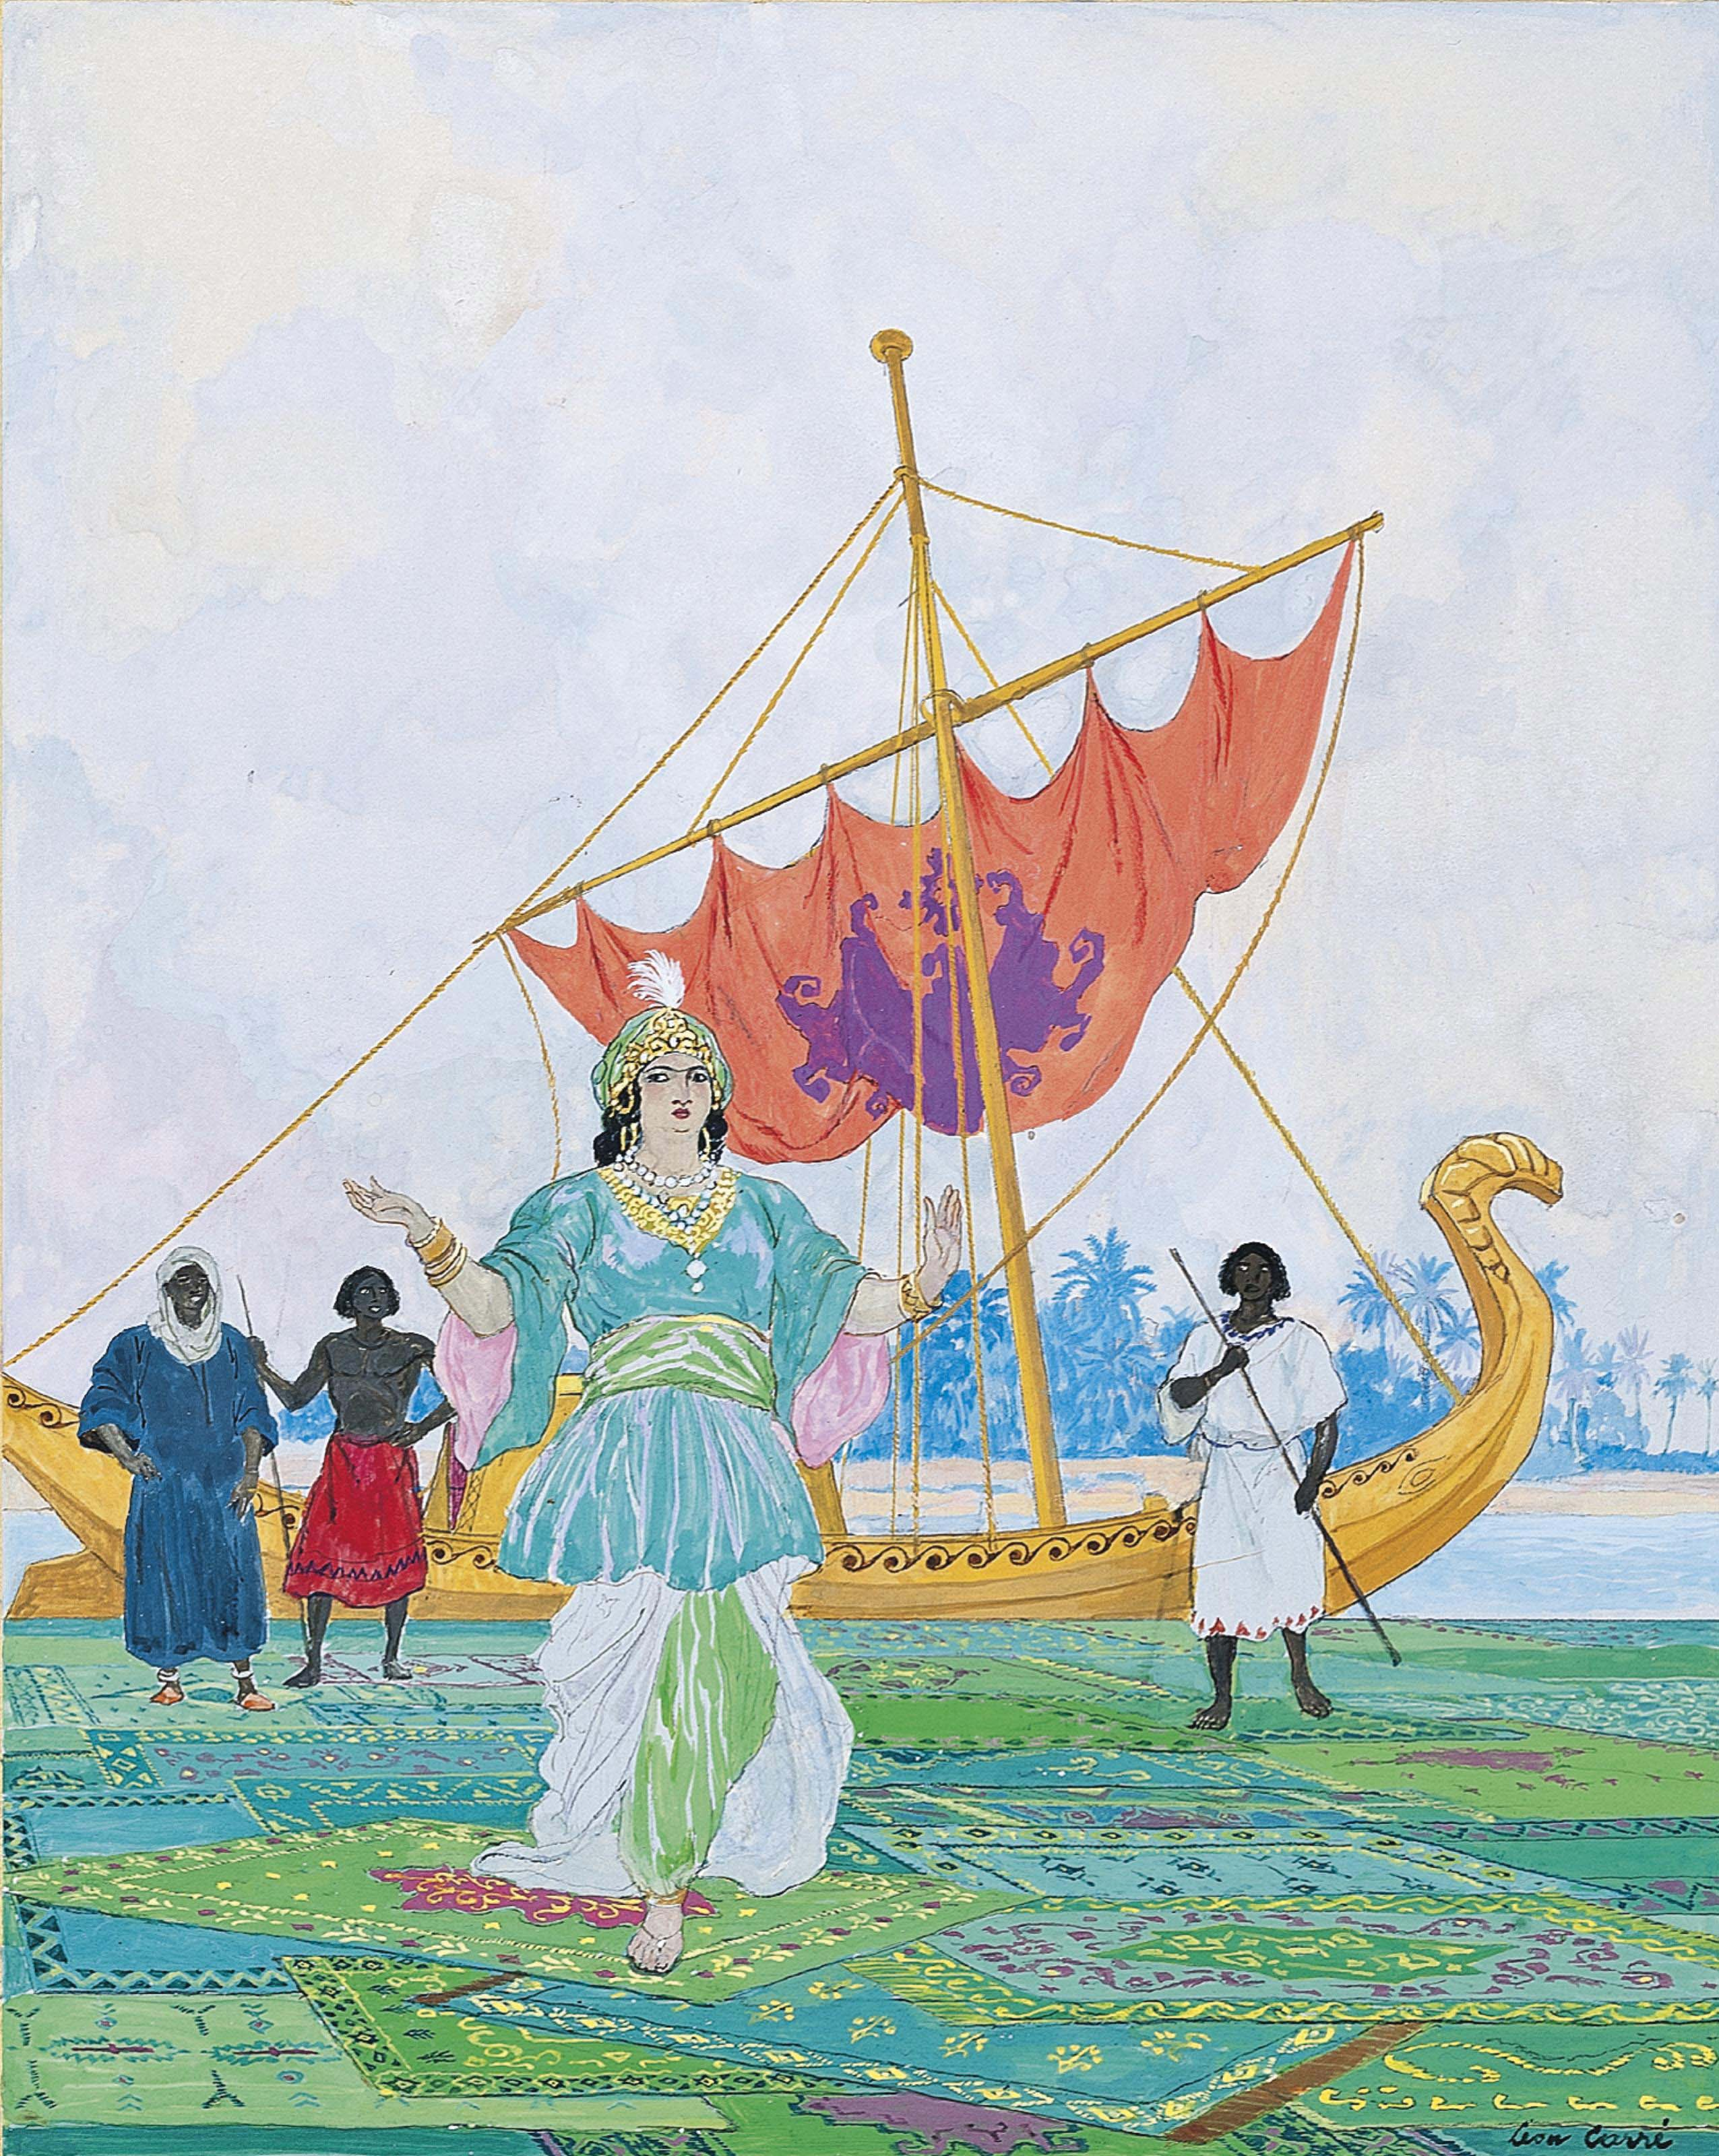
\includegraphics[height=\figsize]{illustrations/volume_8/T08, n0942 - Histoire de Baïbars [Histoire racontée par le quatrième capitaine].jpg}
\end{figure}

\textit{\\
"...la princesse de la Terre Verte sortit de la dahabieh, et marcha sur les tapis de soie, habillée de vert, et se balançant à ravir les esprits."} \\
—T08, n0942 - Histoire de Baïbars [Histoire racontée par le quatrième capitaine] \\~\\
\textit{"...the princess of Green Country came down, clothed all in green, out of the gold boat, and walked, with gentle balancing, over the green silk carpets..."} \\
—V04, n0942 - The tale of Al-Malik Baibars [The fourth captain’s tale]

\newpage

\section{n0948}
\textbf{\Large{The tale of Al-Malik Baibars [The sixth captain’s tale]}} \\

\begin{figure}[ht]
\centering
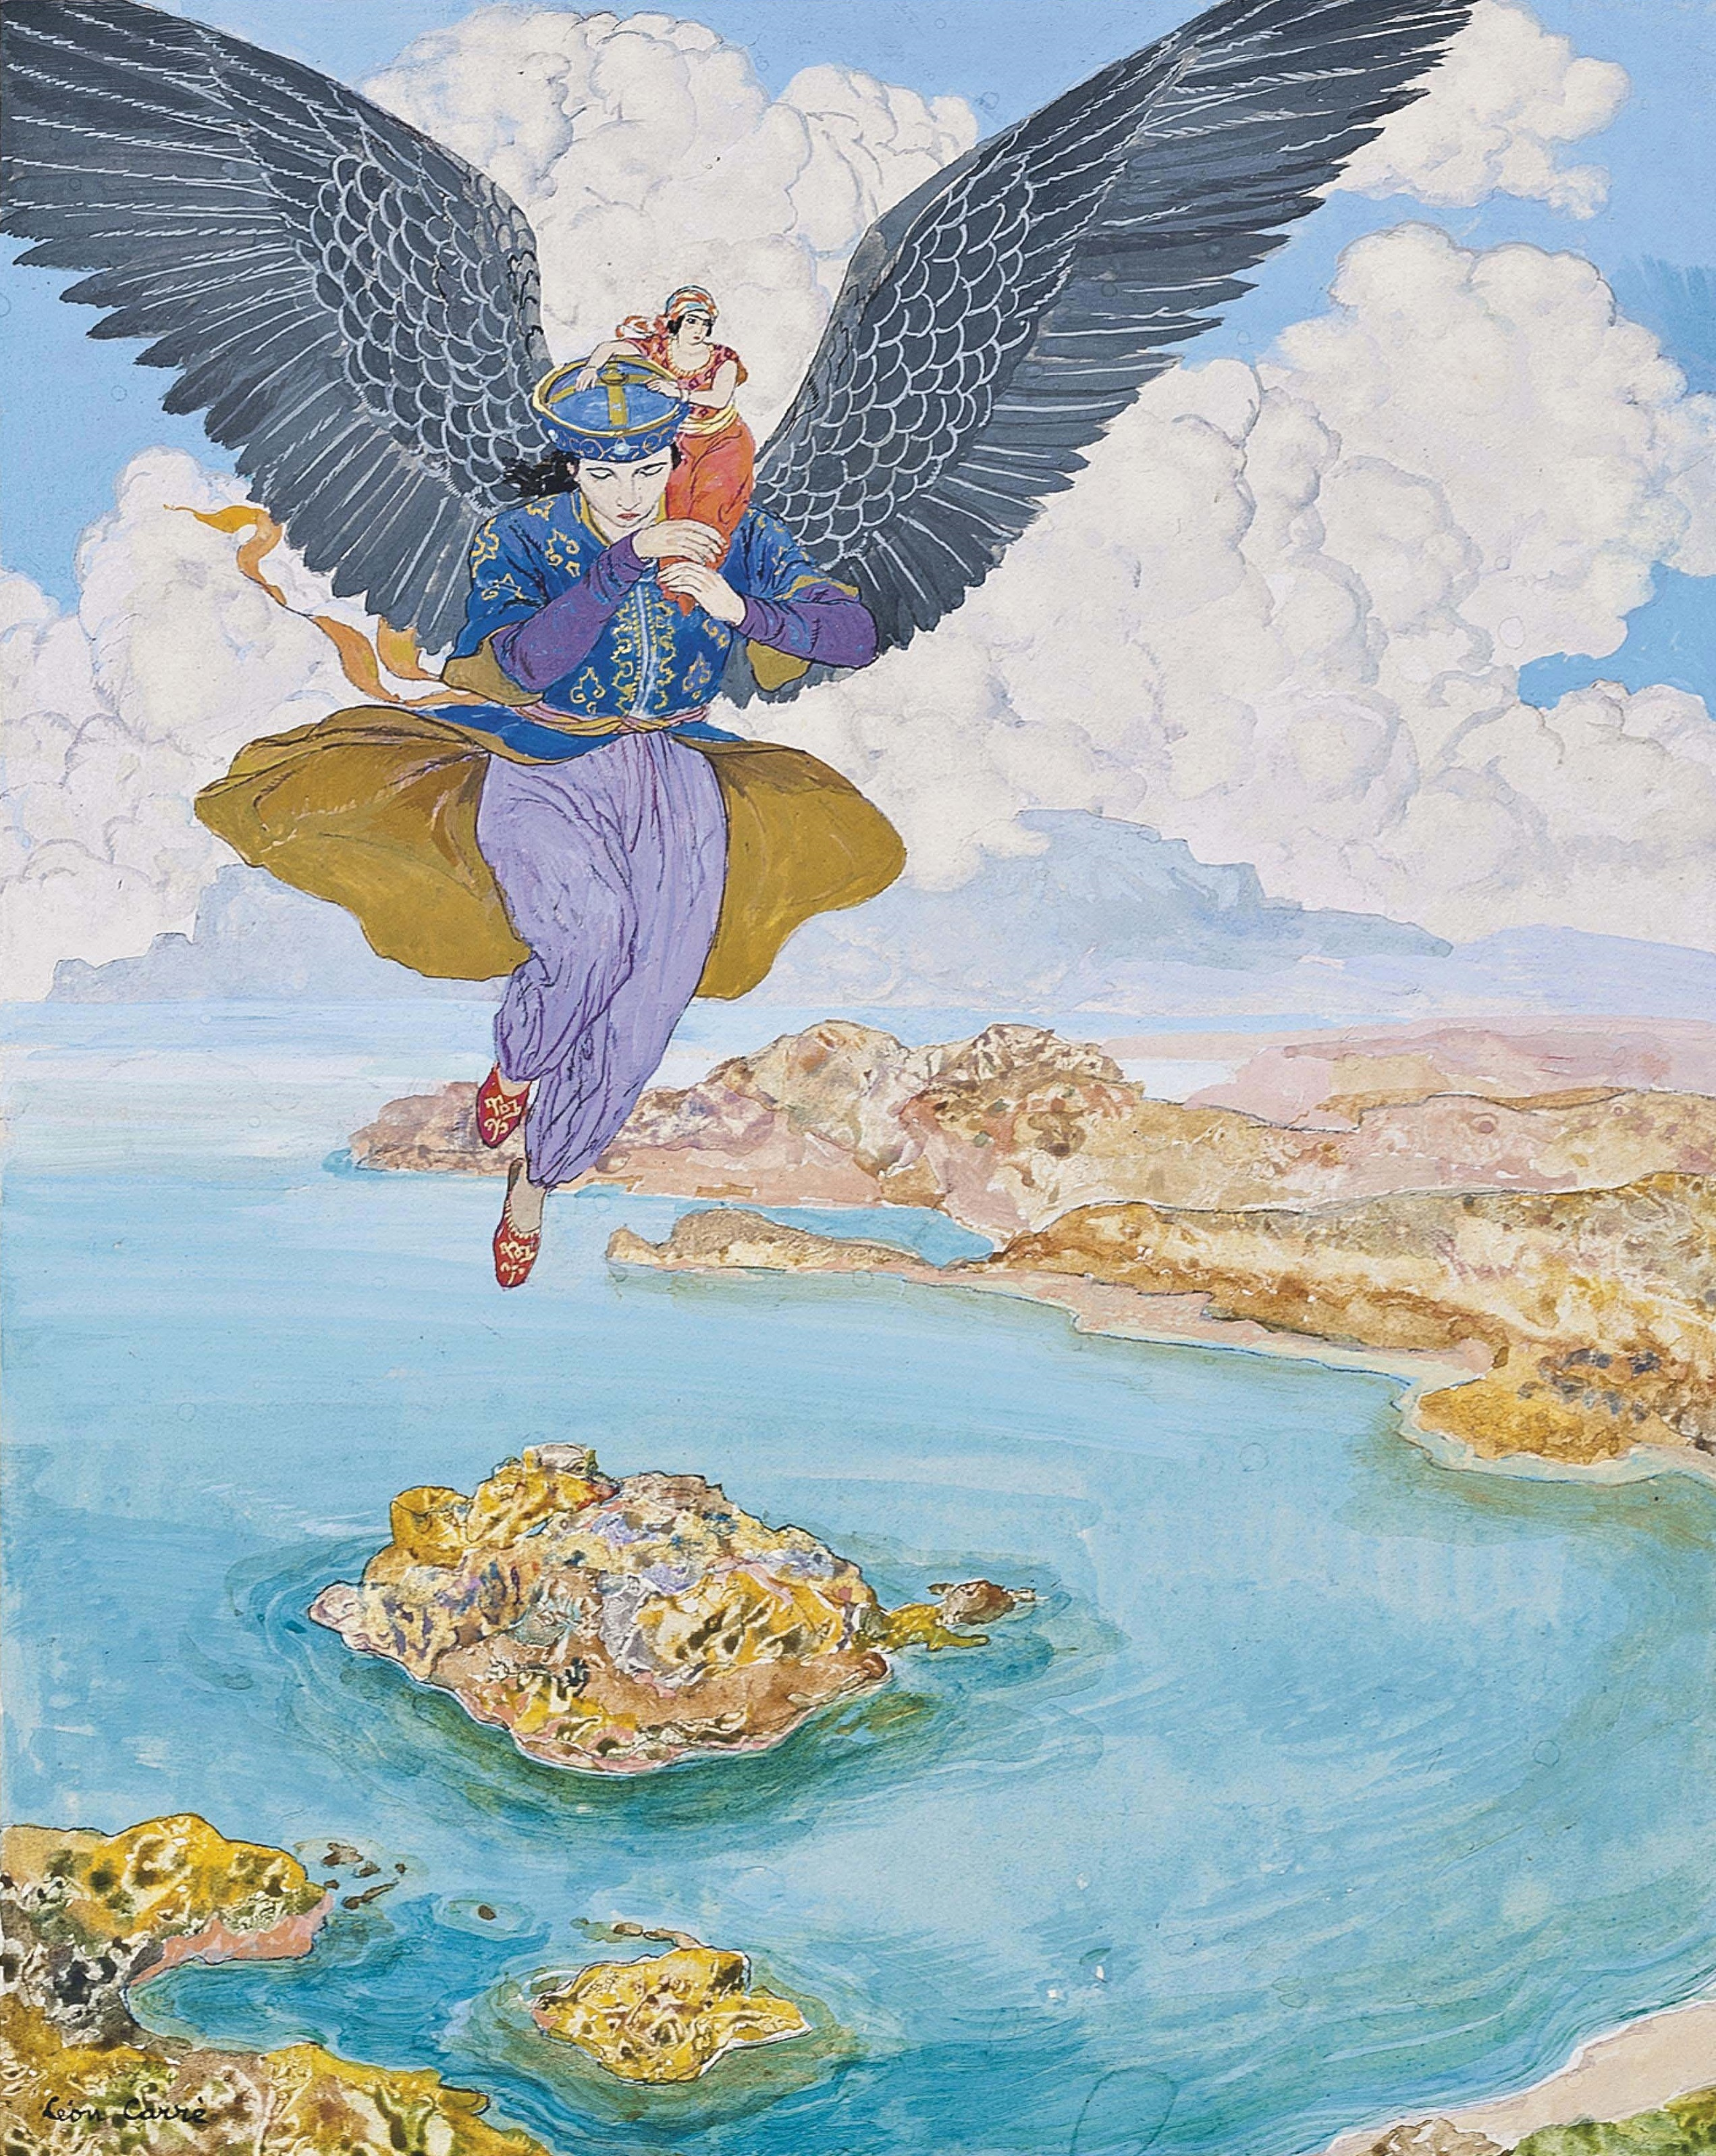
\includegraphics[height=\figsize]{illustrations/volume_8/T08, n0948 - Histoire de Baïbars [Histoire racontée par le sixième capitaine].jpg}
\end{figure}

\textit{\\
"...elle la fit monter sur ses épaules et la porta sur le rivage de la mer d’Émeraude."} \\
—T08, n0948 - Histoire de Baïbars [Histoire racontée par le sixième capitaine] \\~\\
\textit{"The Jinniyah took up Dalal upon her shoulders and carried her to the shores of the Emerald Sea..."} \\
—V04, n0948 - The tale of Al-Malik Baibars [The sixth captain’s tale]

\newpage

\section{n0950}
\textbf{\Large{The tale of Al-Malik Baibars [The ninth captain’s tale]}} \\

\begin{figure}[ht]
\centering
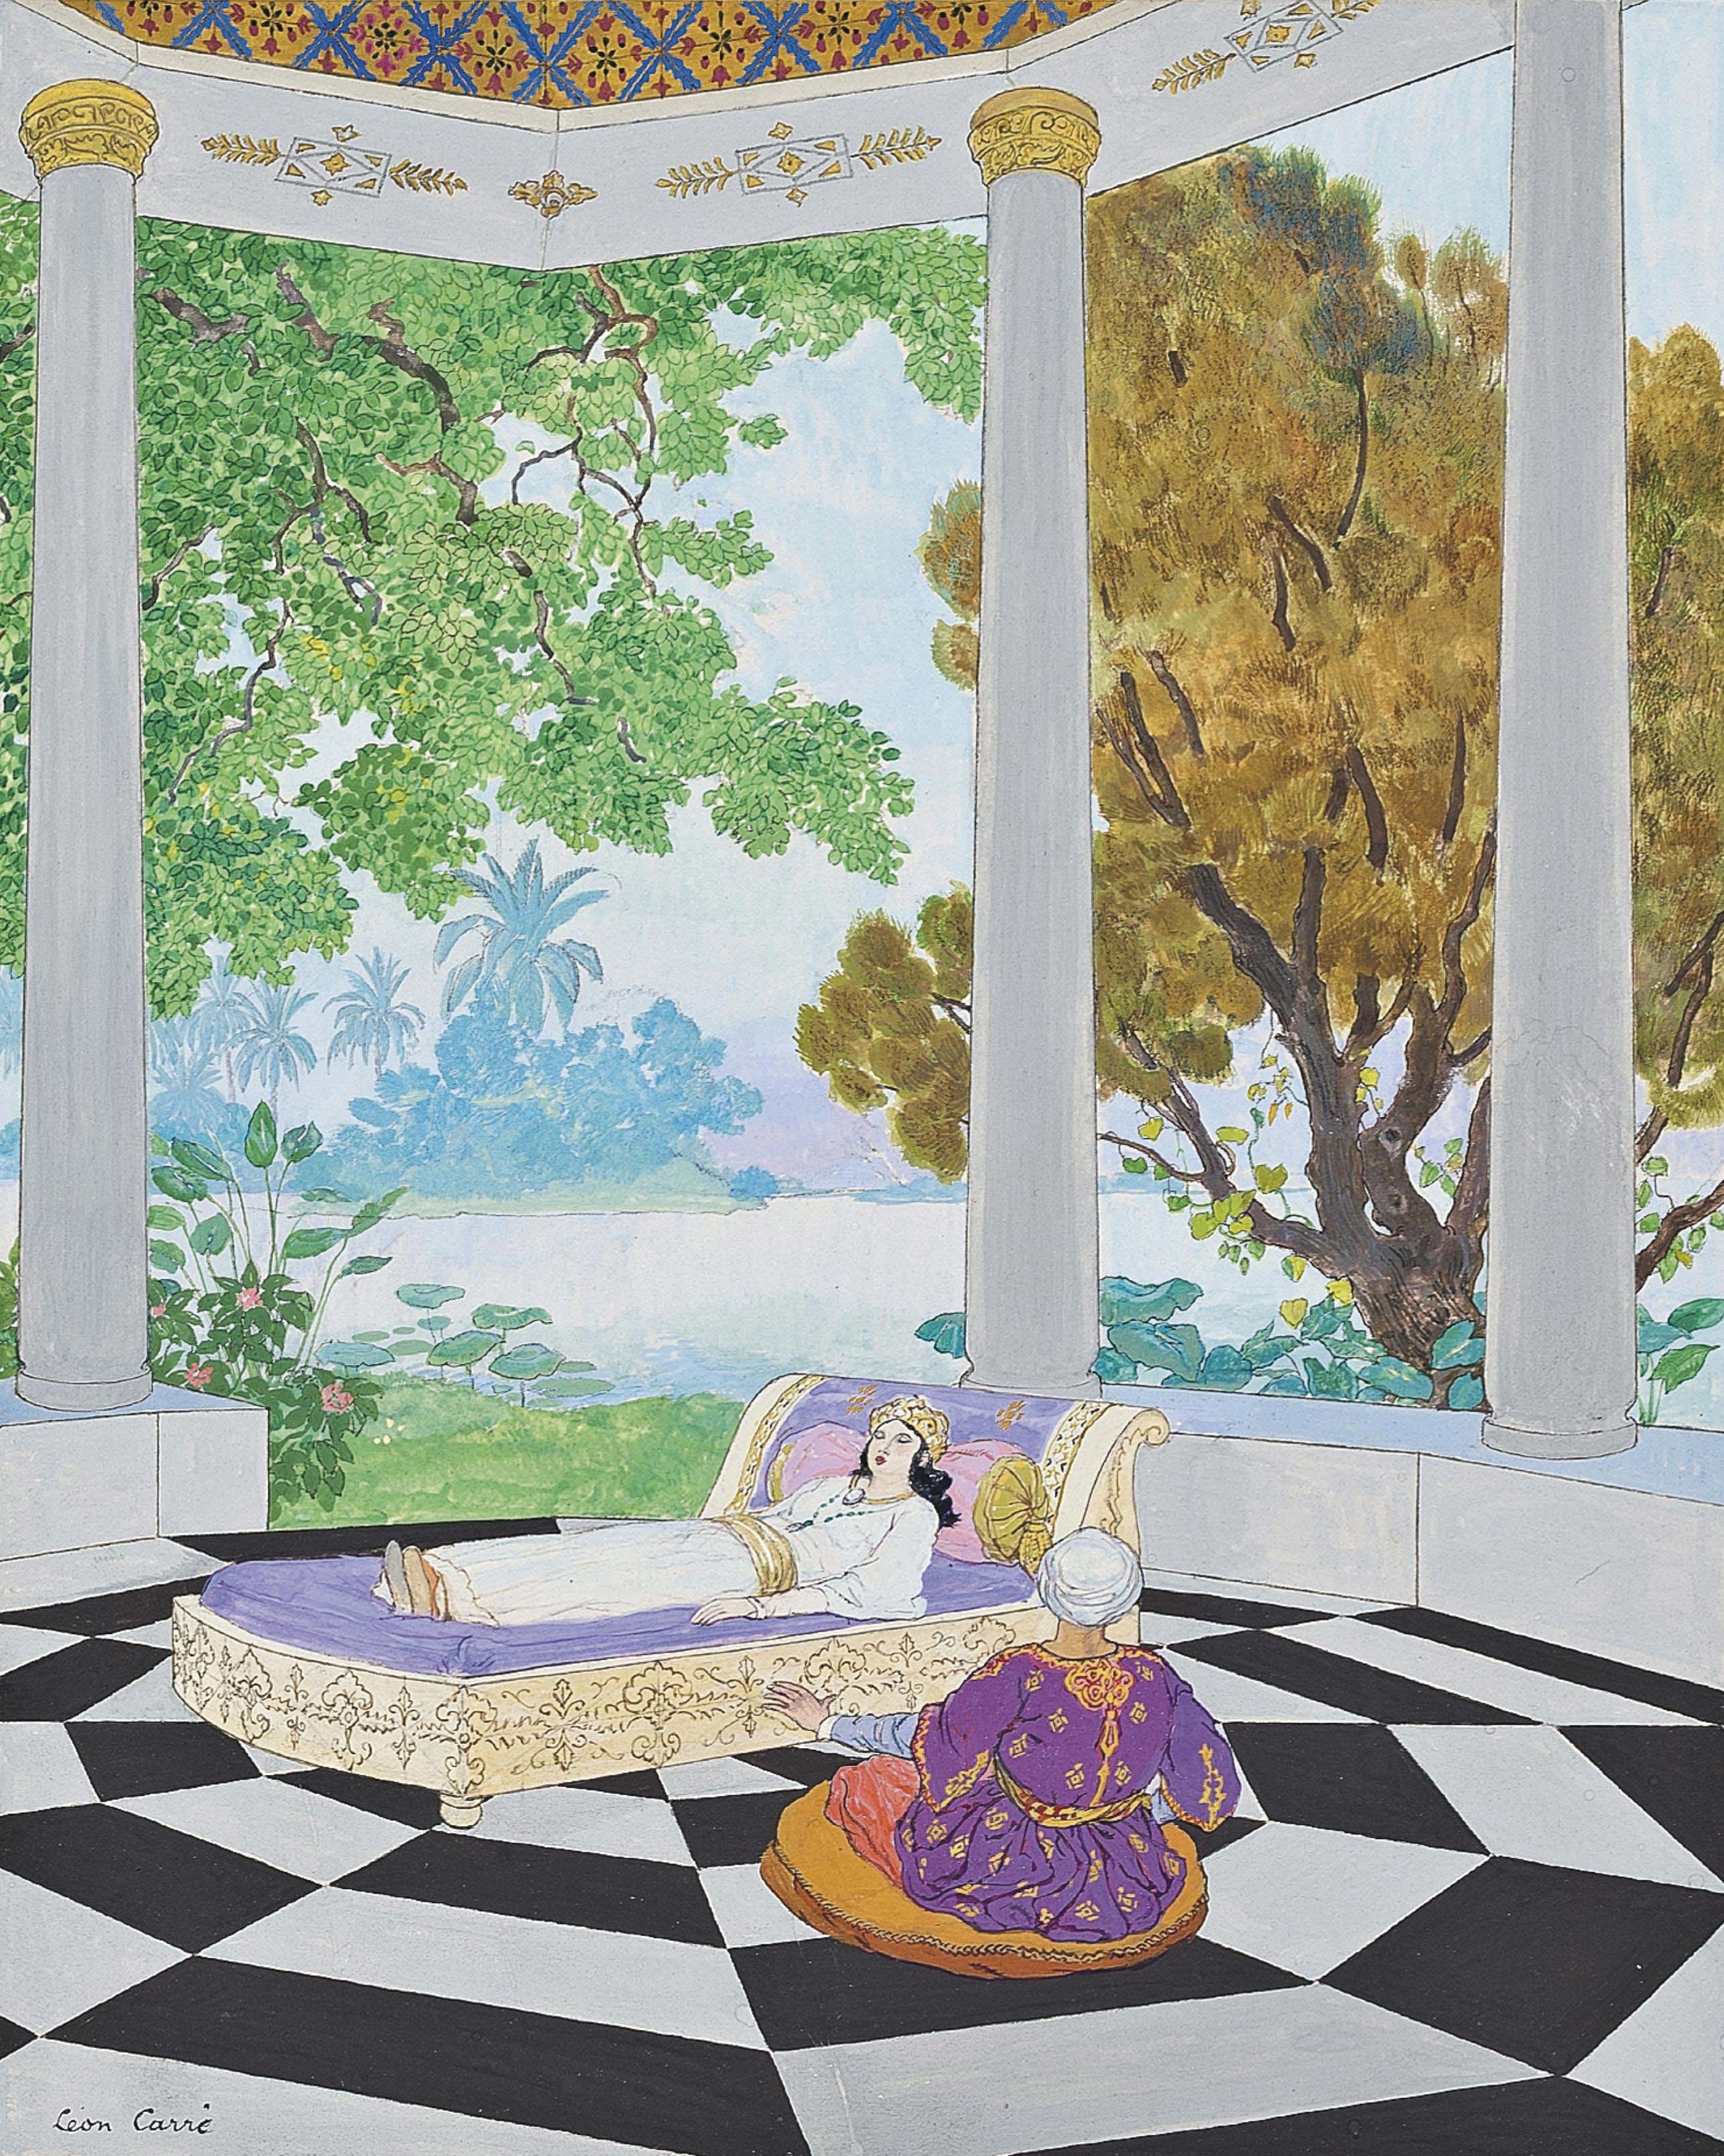
\includegraphics[height=\figsize]{illustrations/volume_8/T08, n0950 - Histoire de Baïbars [Histoire racontée par le neuvième capitaine].jpg}
\end{figure}

\textit{\\
"...il entra dans le pavillon. Et il trouva la jeune fille morte. Et il s’assit à la pleurer, en récitant des vers sur sa beauté."} \\
—T08, n0950 - Histoire de Baïbars [Histoire racontée par le neuvième capitaine] \\~\\
\textit{"He entered the pavilion and began to weep by the ivory bed, recalling verses in the praise of so much beauty."} \\
—V04, n0950 - The tale of Al-Malik Baibars [The ninth captain’s tale]

\newpage

\section{n0955}
\textbf{\Large{The tale of the sea rose of the girl of China}} \\

\begin{figure}[ht]
\centering
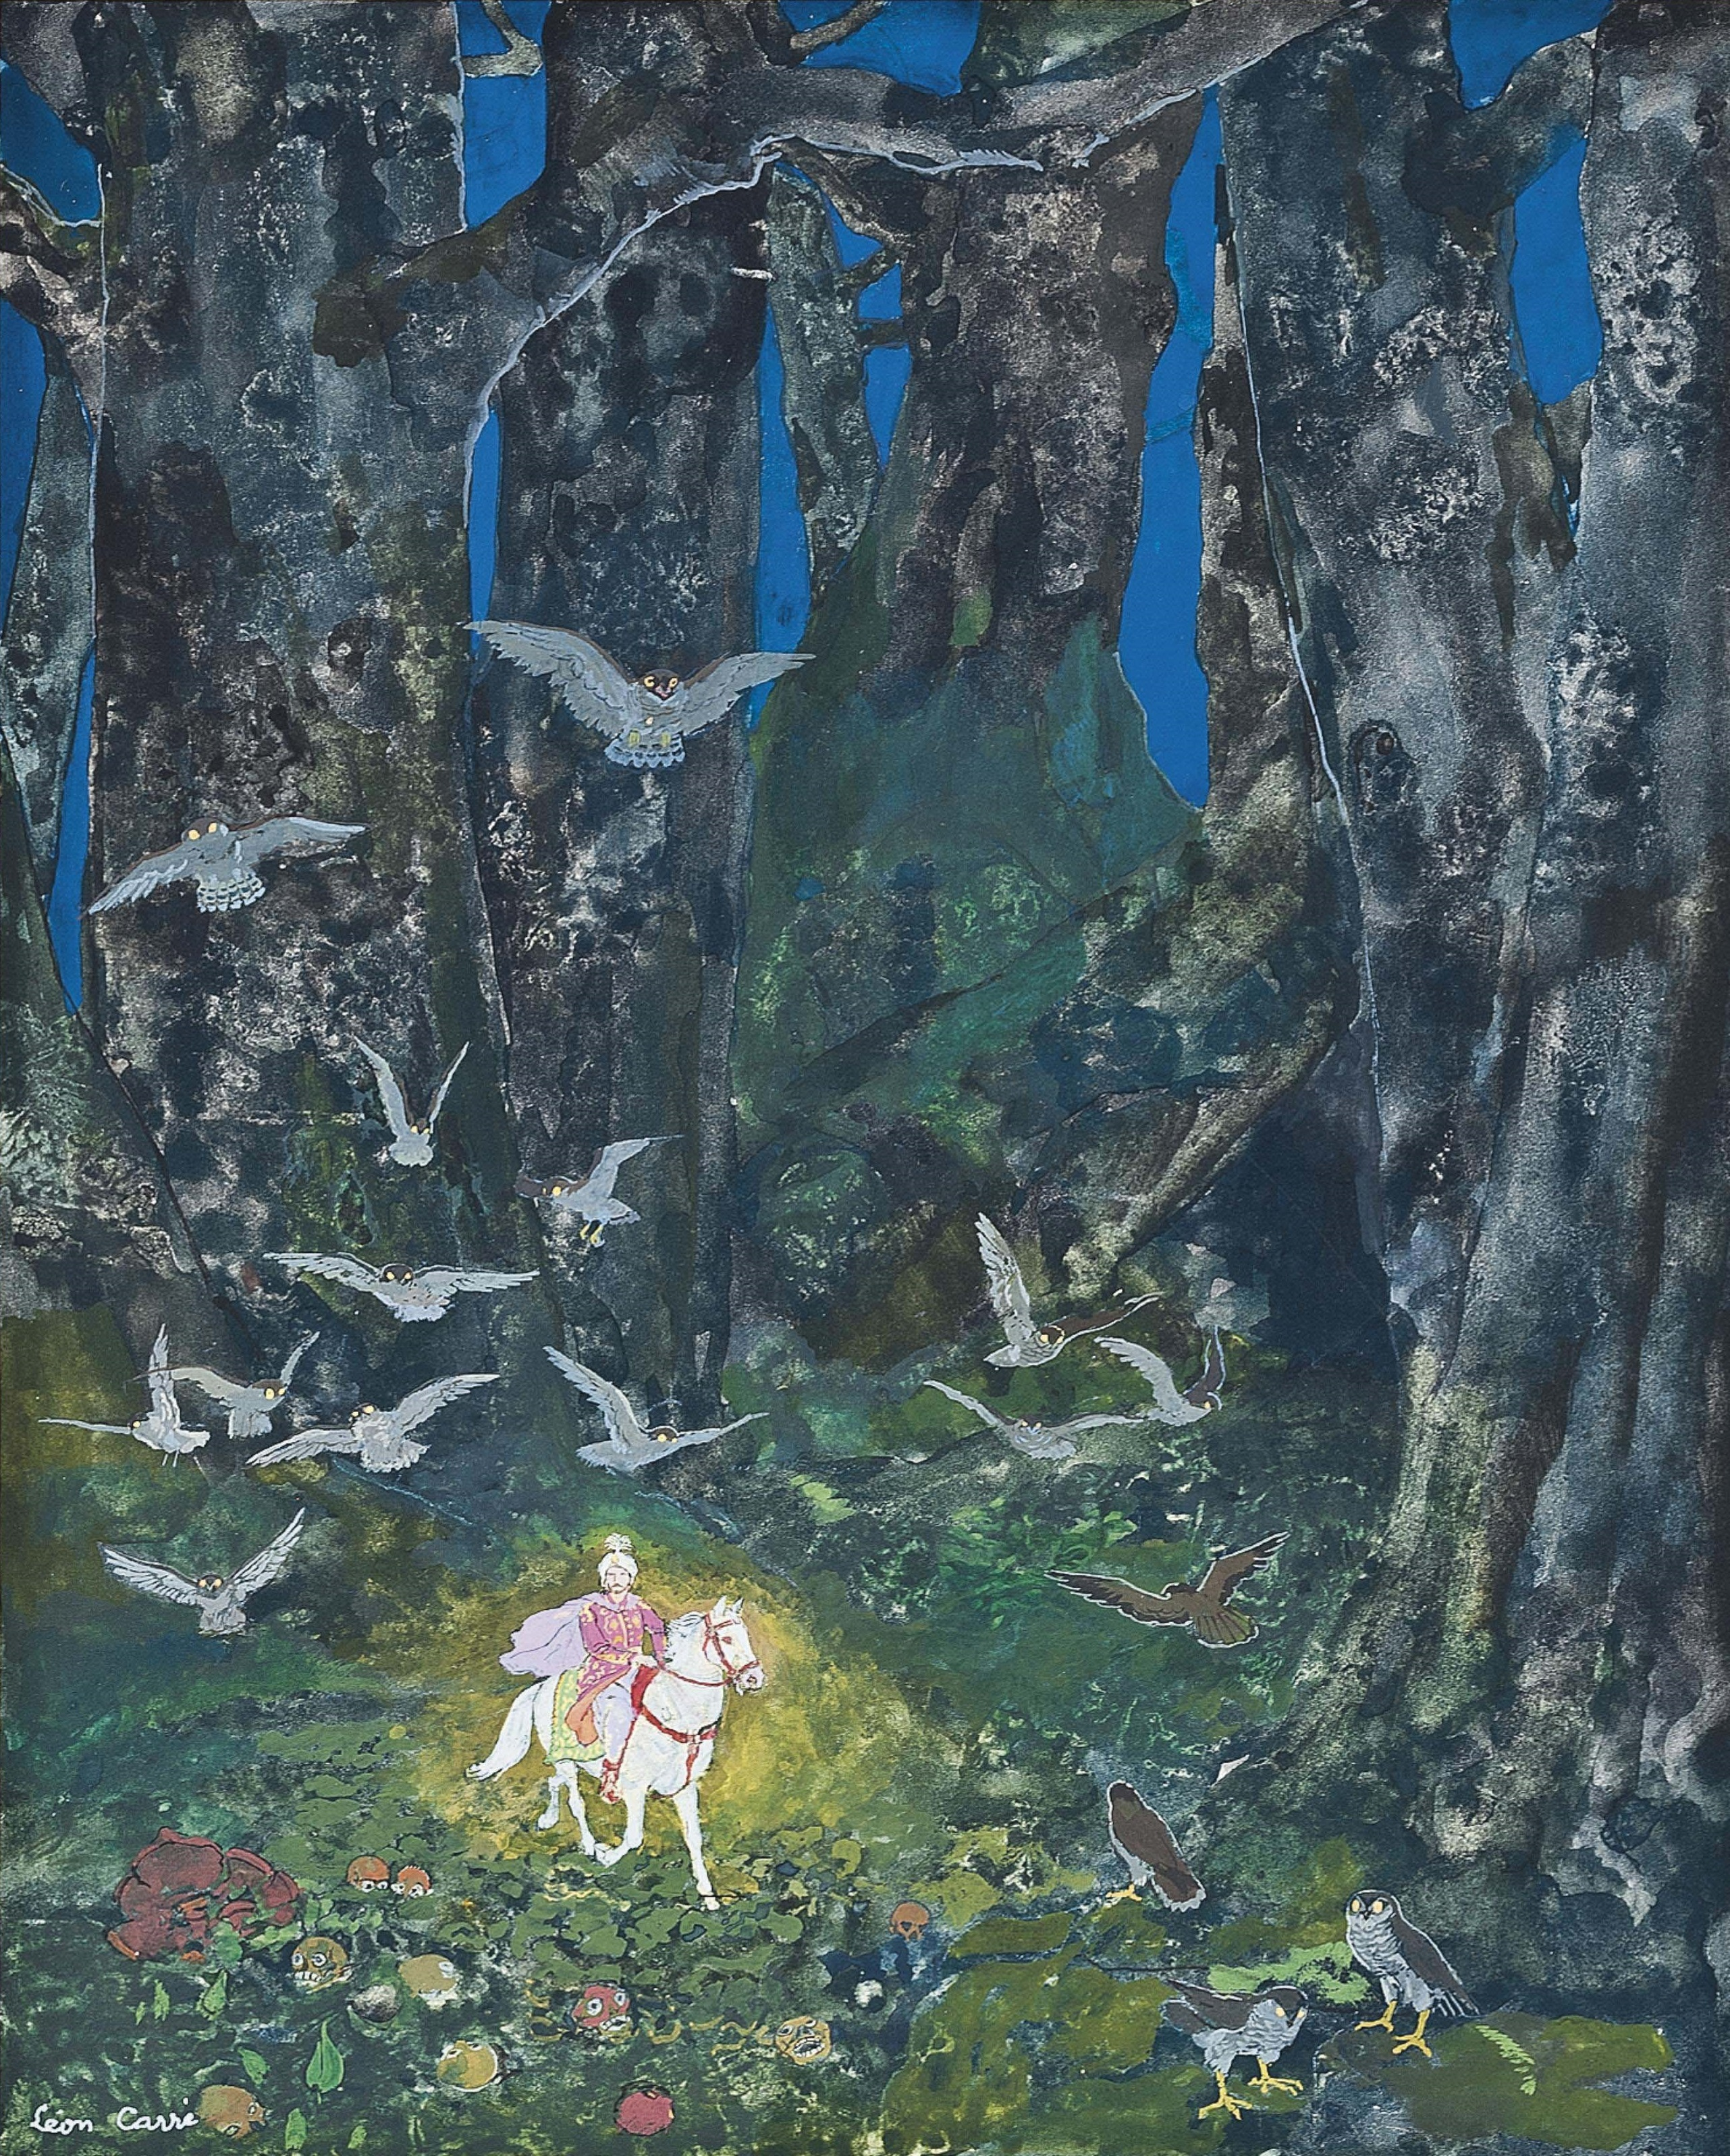
\includegraphics[height=\figsize]{illustrations/volume_8/T08, n0955 - Histoire de la rose marine et de l'adolescente de Chine.jpg}
\end{figure}

\textit{\\
"...Nourgihân, dont le brillant visage éclairait seul les ténèbres, s’avançait d’un cœur d’acier dans cette forêt dont les arbres portaient, par endroits, en guise de fruits, des têtes d’êtres animés qui se mettaient à ricaner et à rire et tombaient par terre..."} \\
—T08, n0955 - Histoire de la rose marine et de l'adolescente de Chine \\~\\
\textit{"...the prince's shining face lit up the shadows, and he advanced, with a heart of steel, among trees bearing living heads which grinned and laughed and fell as he passed by..."} \\
—V04, n0955 - The tale of the sea rose of the girl of China

\newpage

\section{n0958}
\textbf{\Large{The tale of the sea rose of the girl of China}} \\

\begin{figure}[ht]
\centering
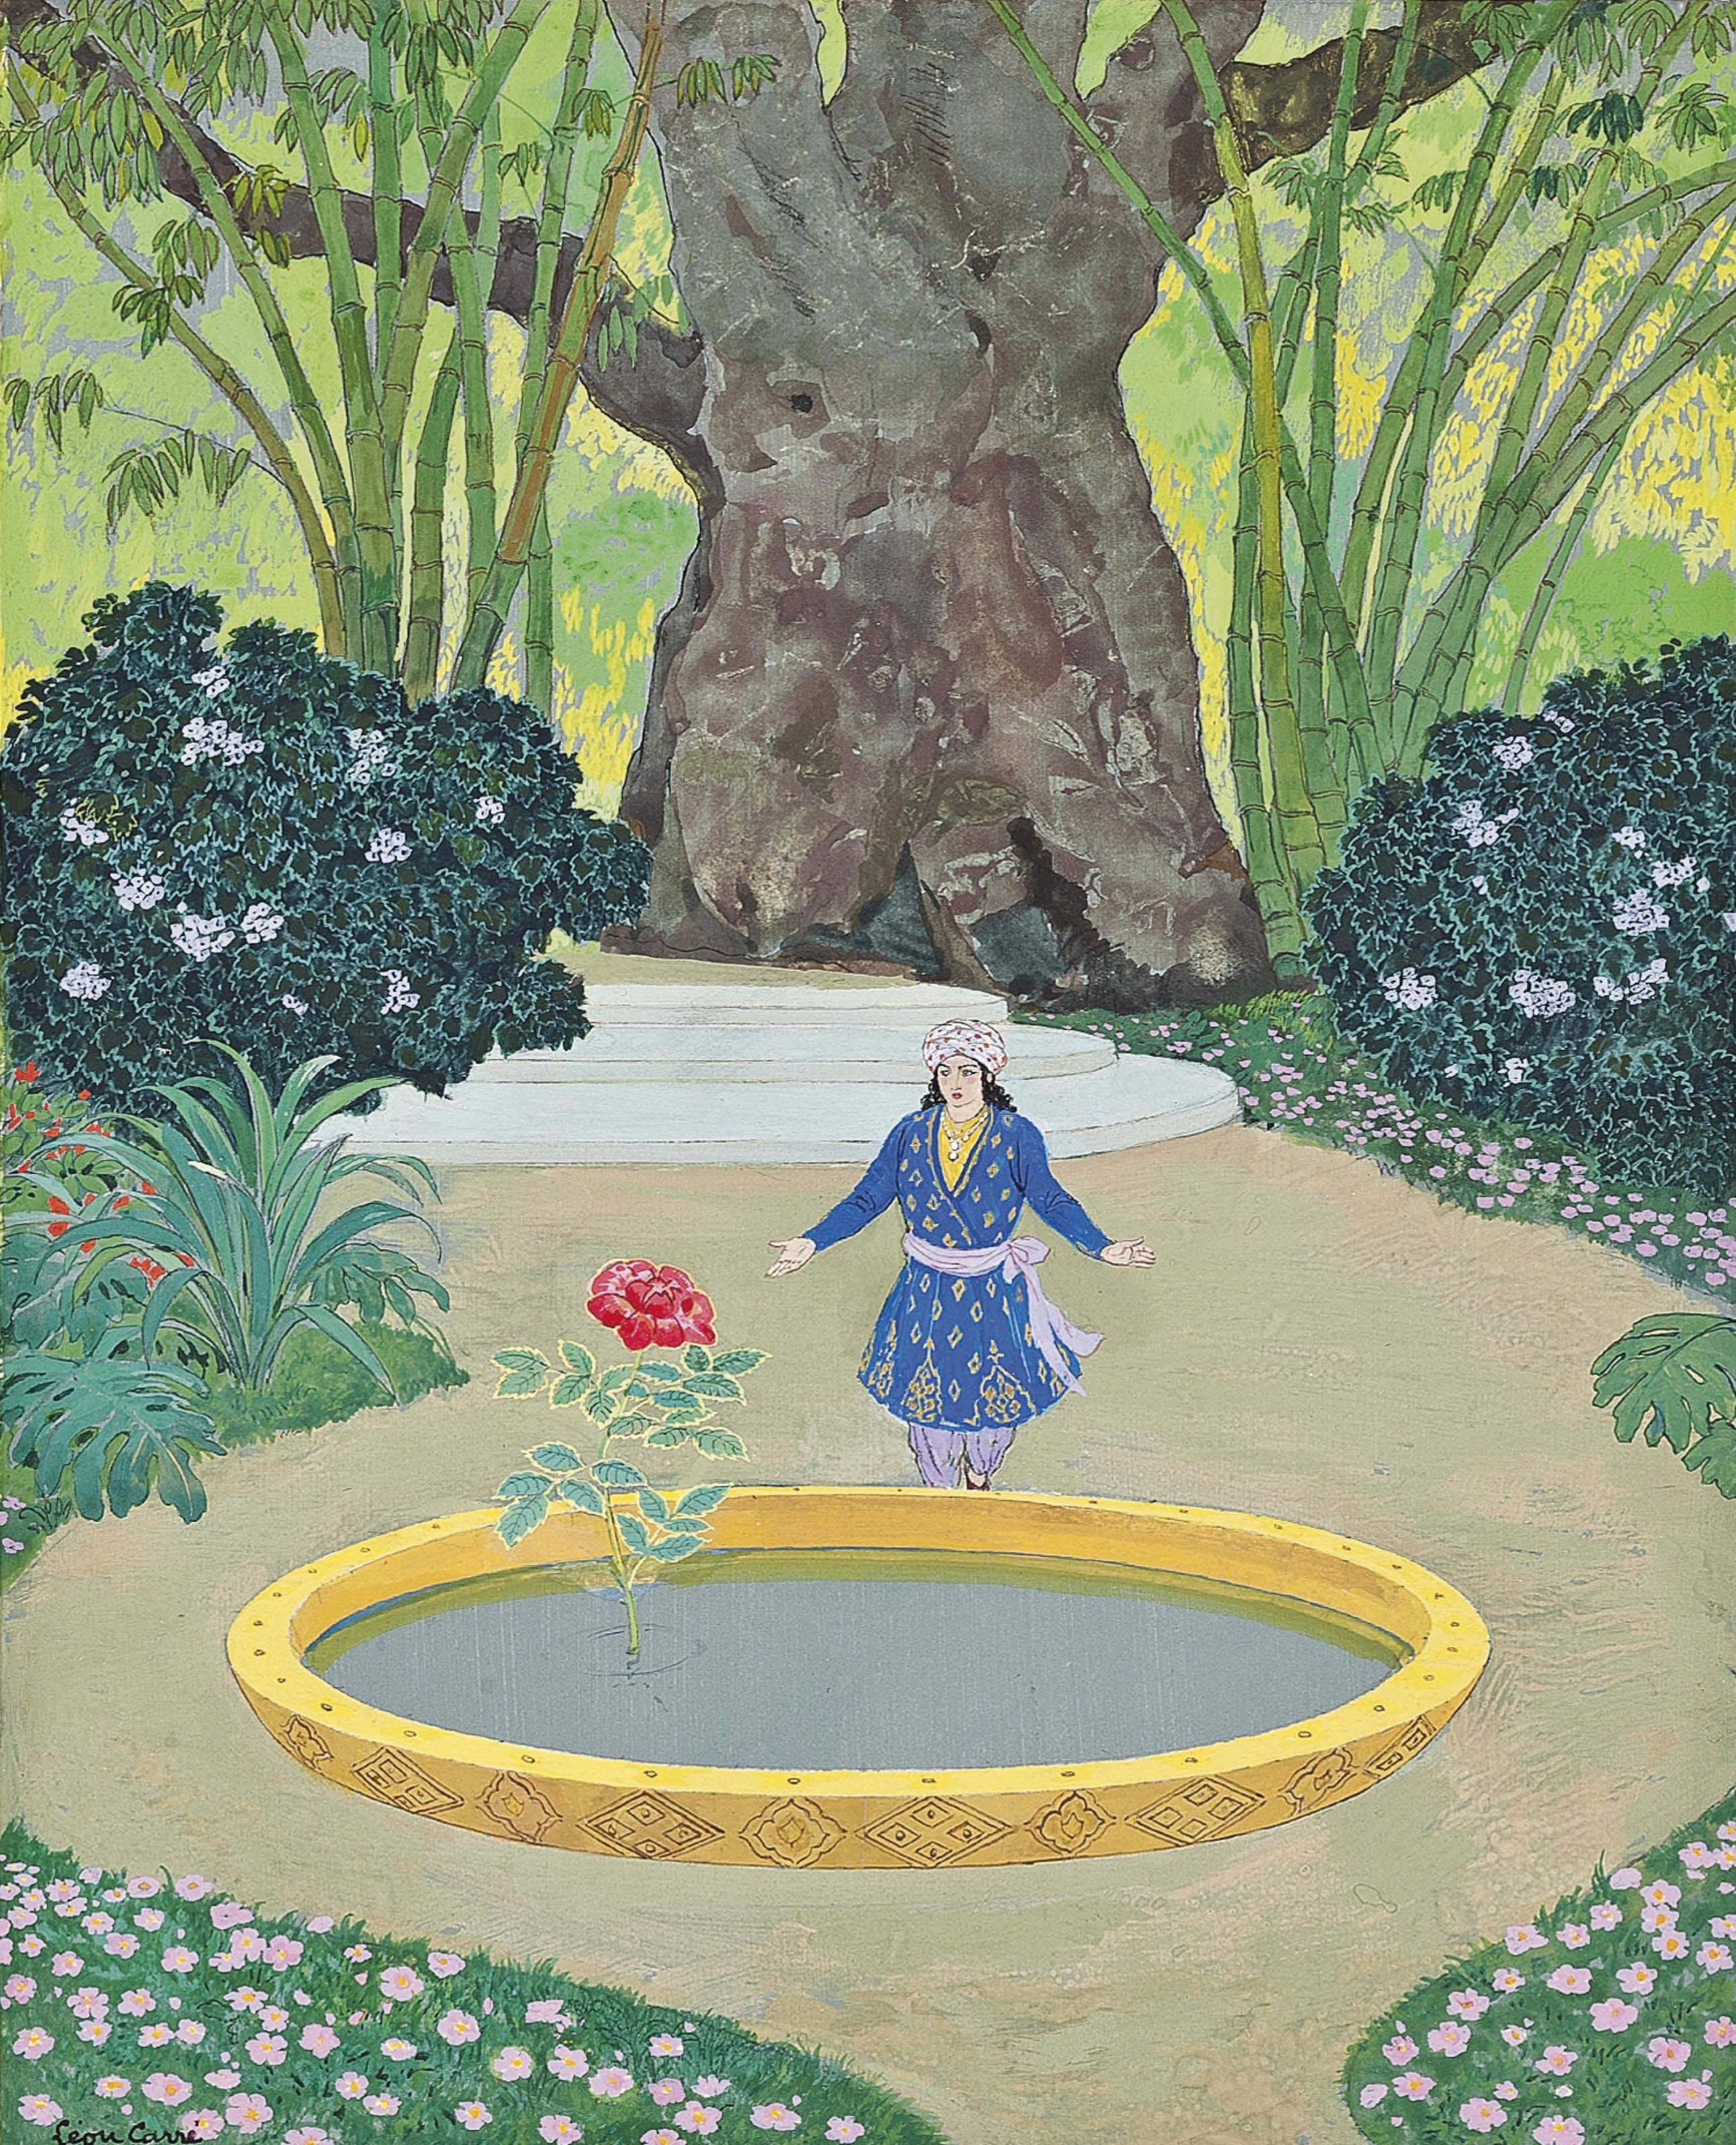
\includegraphics[height=\figsize]{illustrations/volume_8/T08, n0958 - Histoire de la rose marine et de l'adolescente de Chine.jpg}
\end{figure}

\textit{\\
"...elle arriva ainsi au jardin, et vit, dans le bassin d’or pur, sa rose marine épanouie comme jadis, au milieu de l’eau précieuse des roses, enchantement pour les yeux et baume pour l’odorat."} \\
—T08, n0958 - Histoire de la rose marine et de l'adolescente de Chine \\~\\
\textit{"...she came to the royal garden and saw the sea rose blossoming, as of old, in the scented water of its gold pond."} \\
—V04, n0958 - The tale of the sea rose of the girl of China

\newpage

\section{n0963}
\textbf{\Large{The tale of the honey cake}} \\

\begin{figure}[ht]
\centering
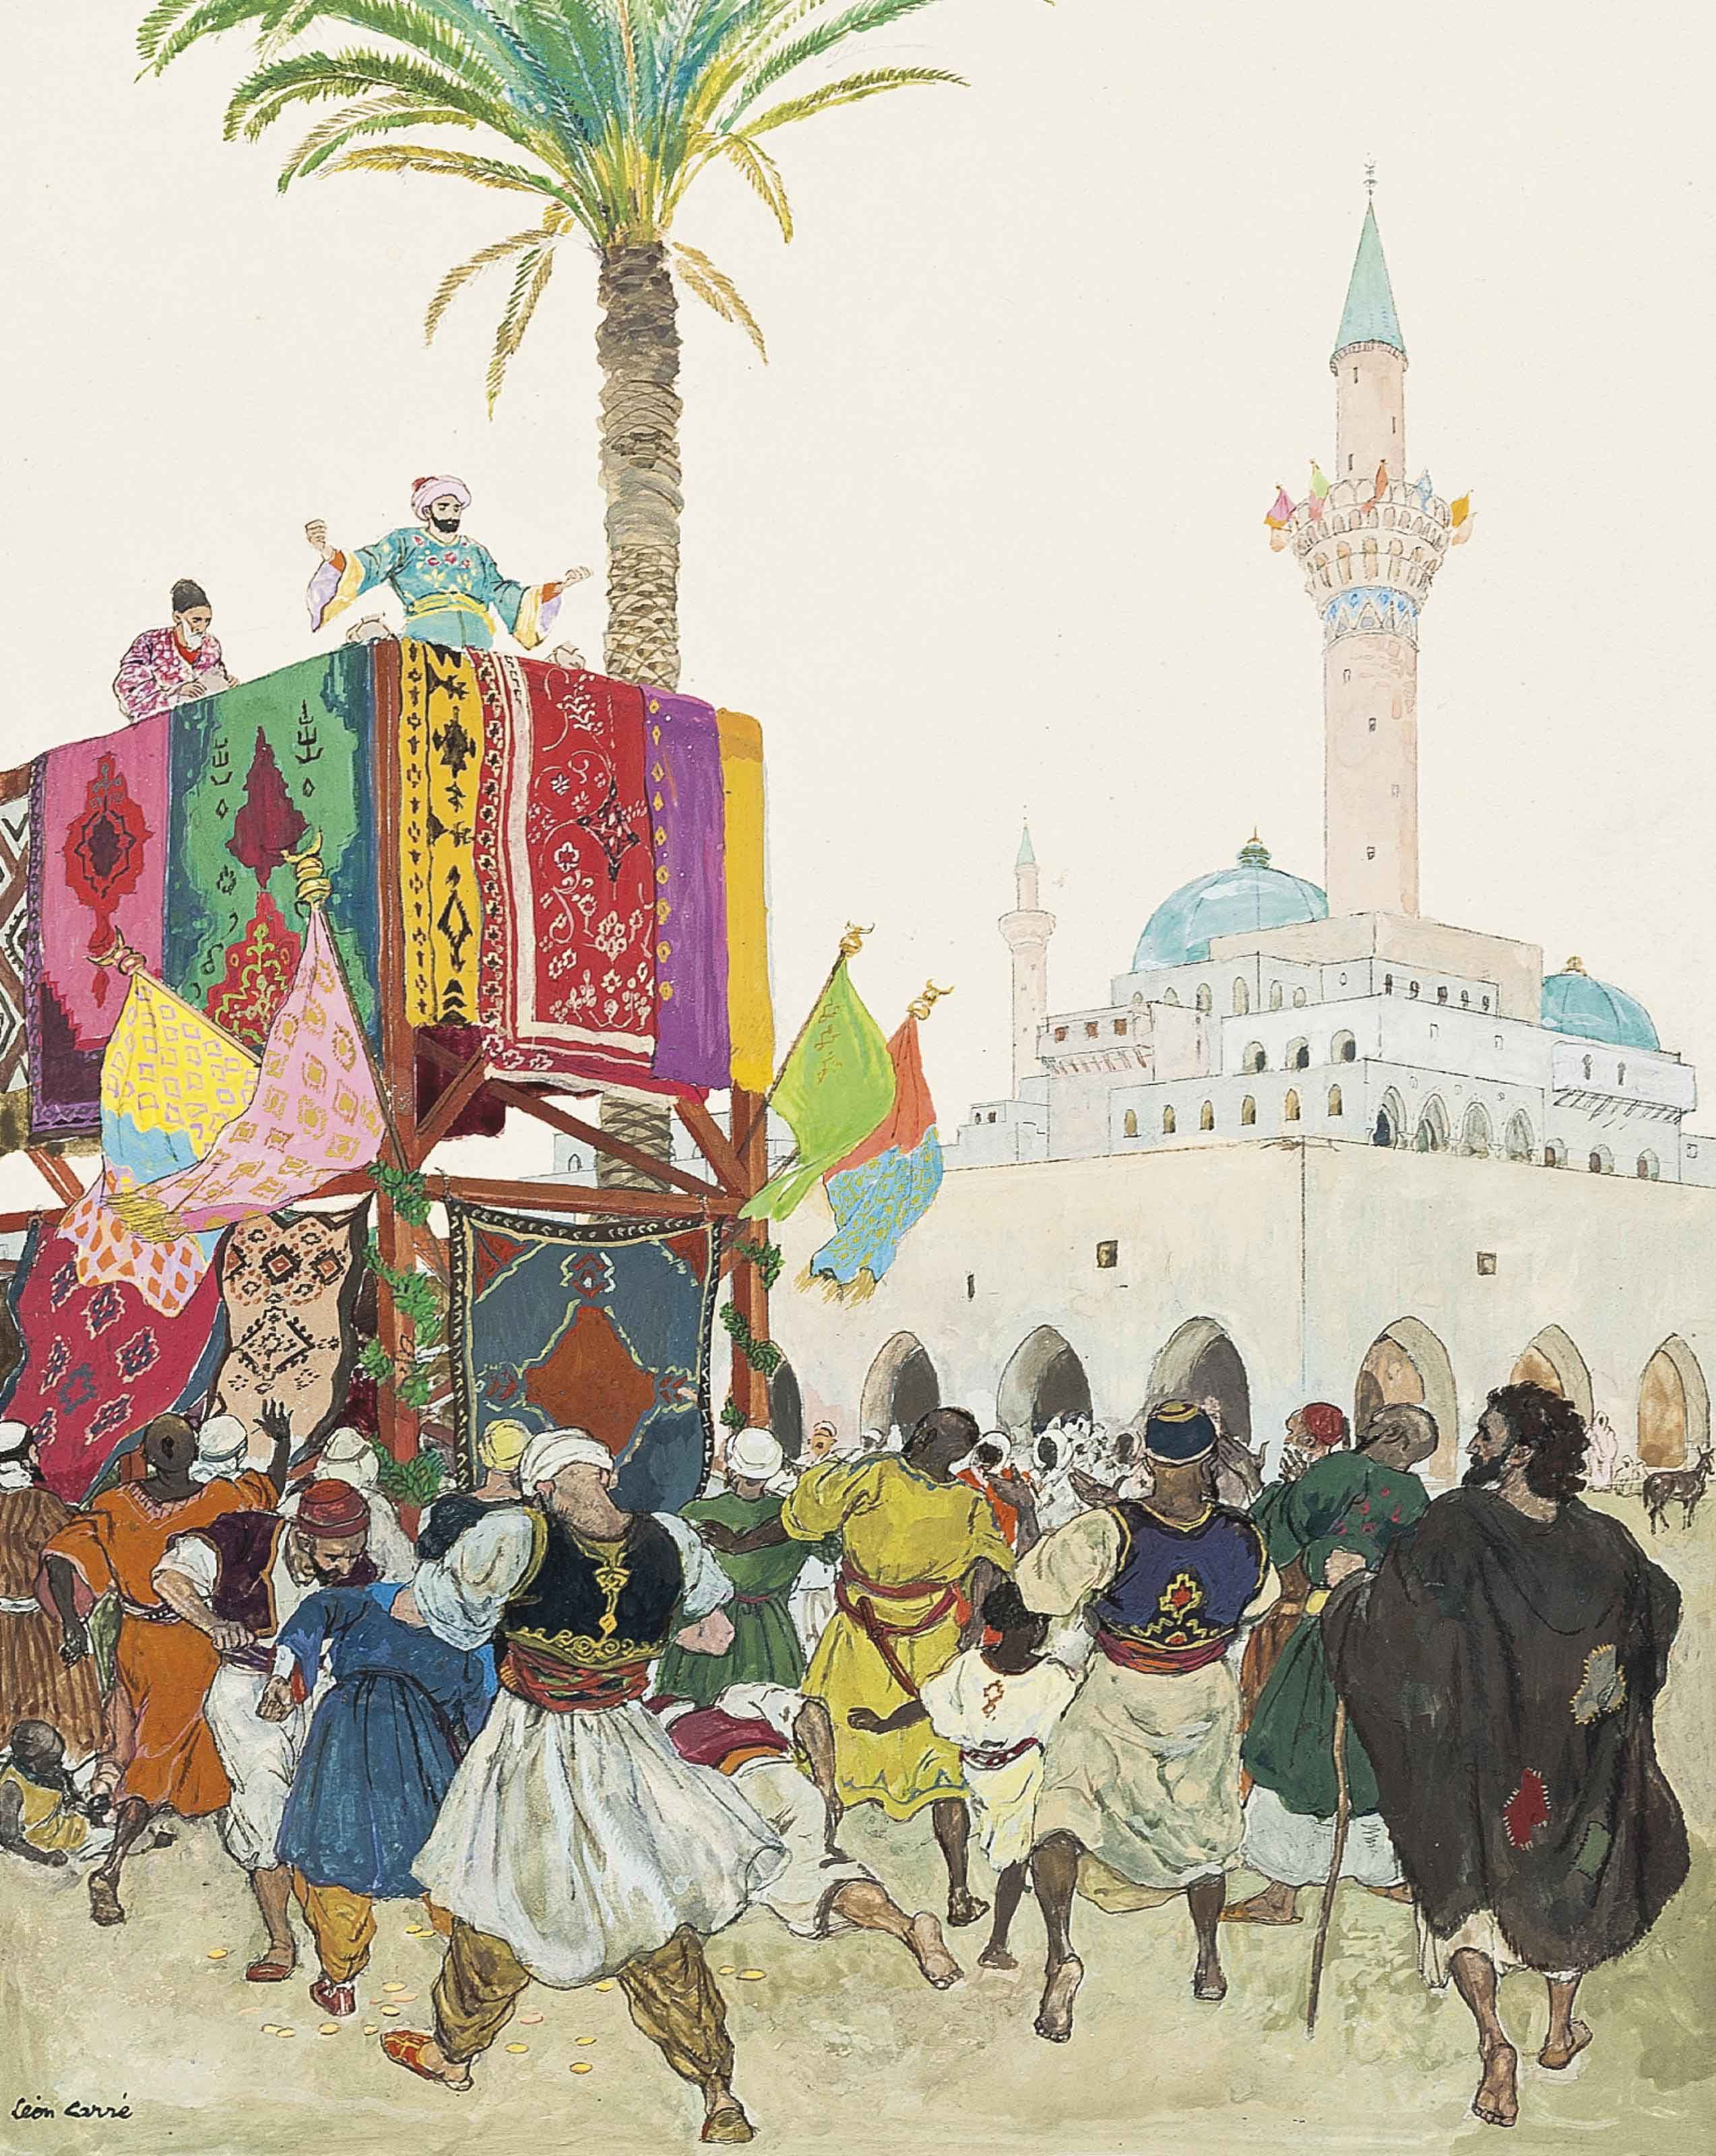
\includegraphics[height=\figsize]{illustrations/volume_8/T08, n0963 - Histoire du gateau échevelé au miel d'abeilles.jpg}
\end{figure}

\textit{\\
"...Mârouf se fit apporter, par le vizir lui-même, des sacs et des sacs pleins d’or, et se mit à prendre les dinars et à les jeter par poignées à tout ce peuple tambourinant, dansant et tintamarrant."} \\
—T08, n0963 - Histoire du gateau échevelé au miel d'abeilles \\~\\
\textit{"...Maaruf had the wazir bring sack after sack of gold to cast among the shouting, singing, dancing mob."} \\
—V04, n0963 - The tale of the honey cake

\newpage

\section{n0969}
\textbf{\Large{The tale of the honey cake}} \\

\begin{figure}[ht]
\centering
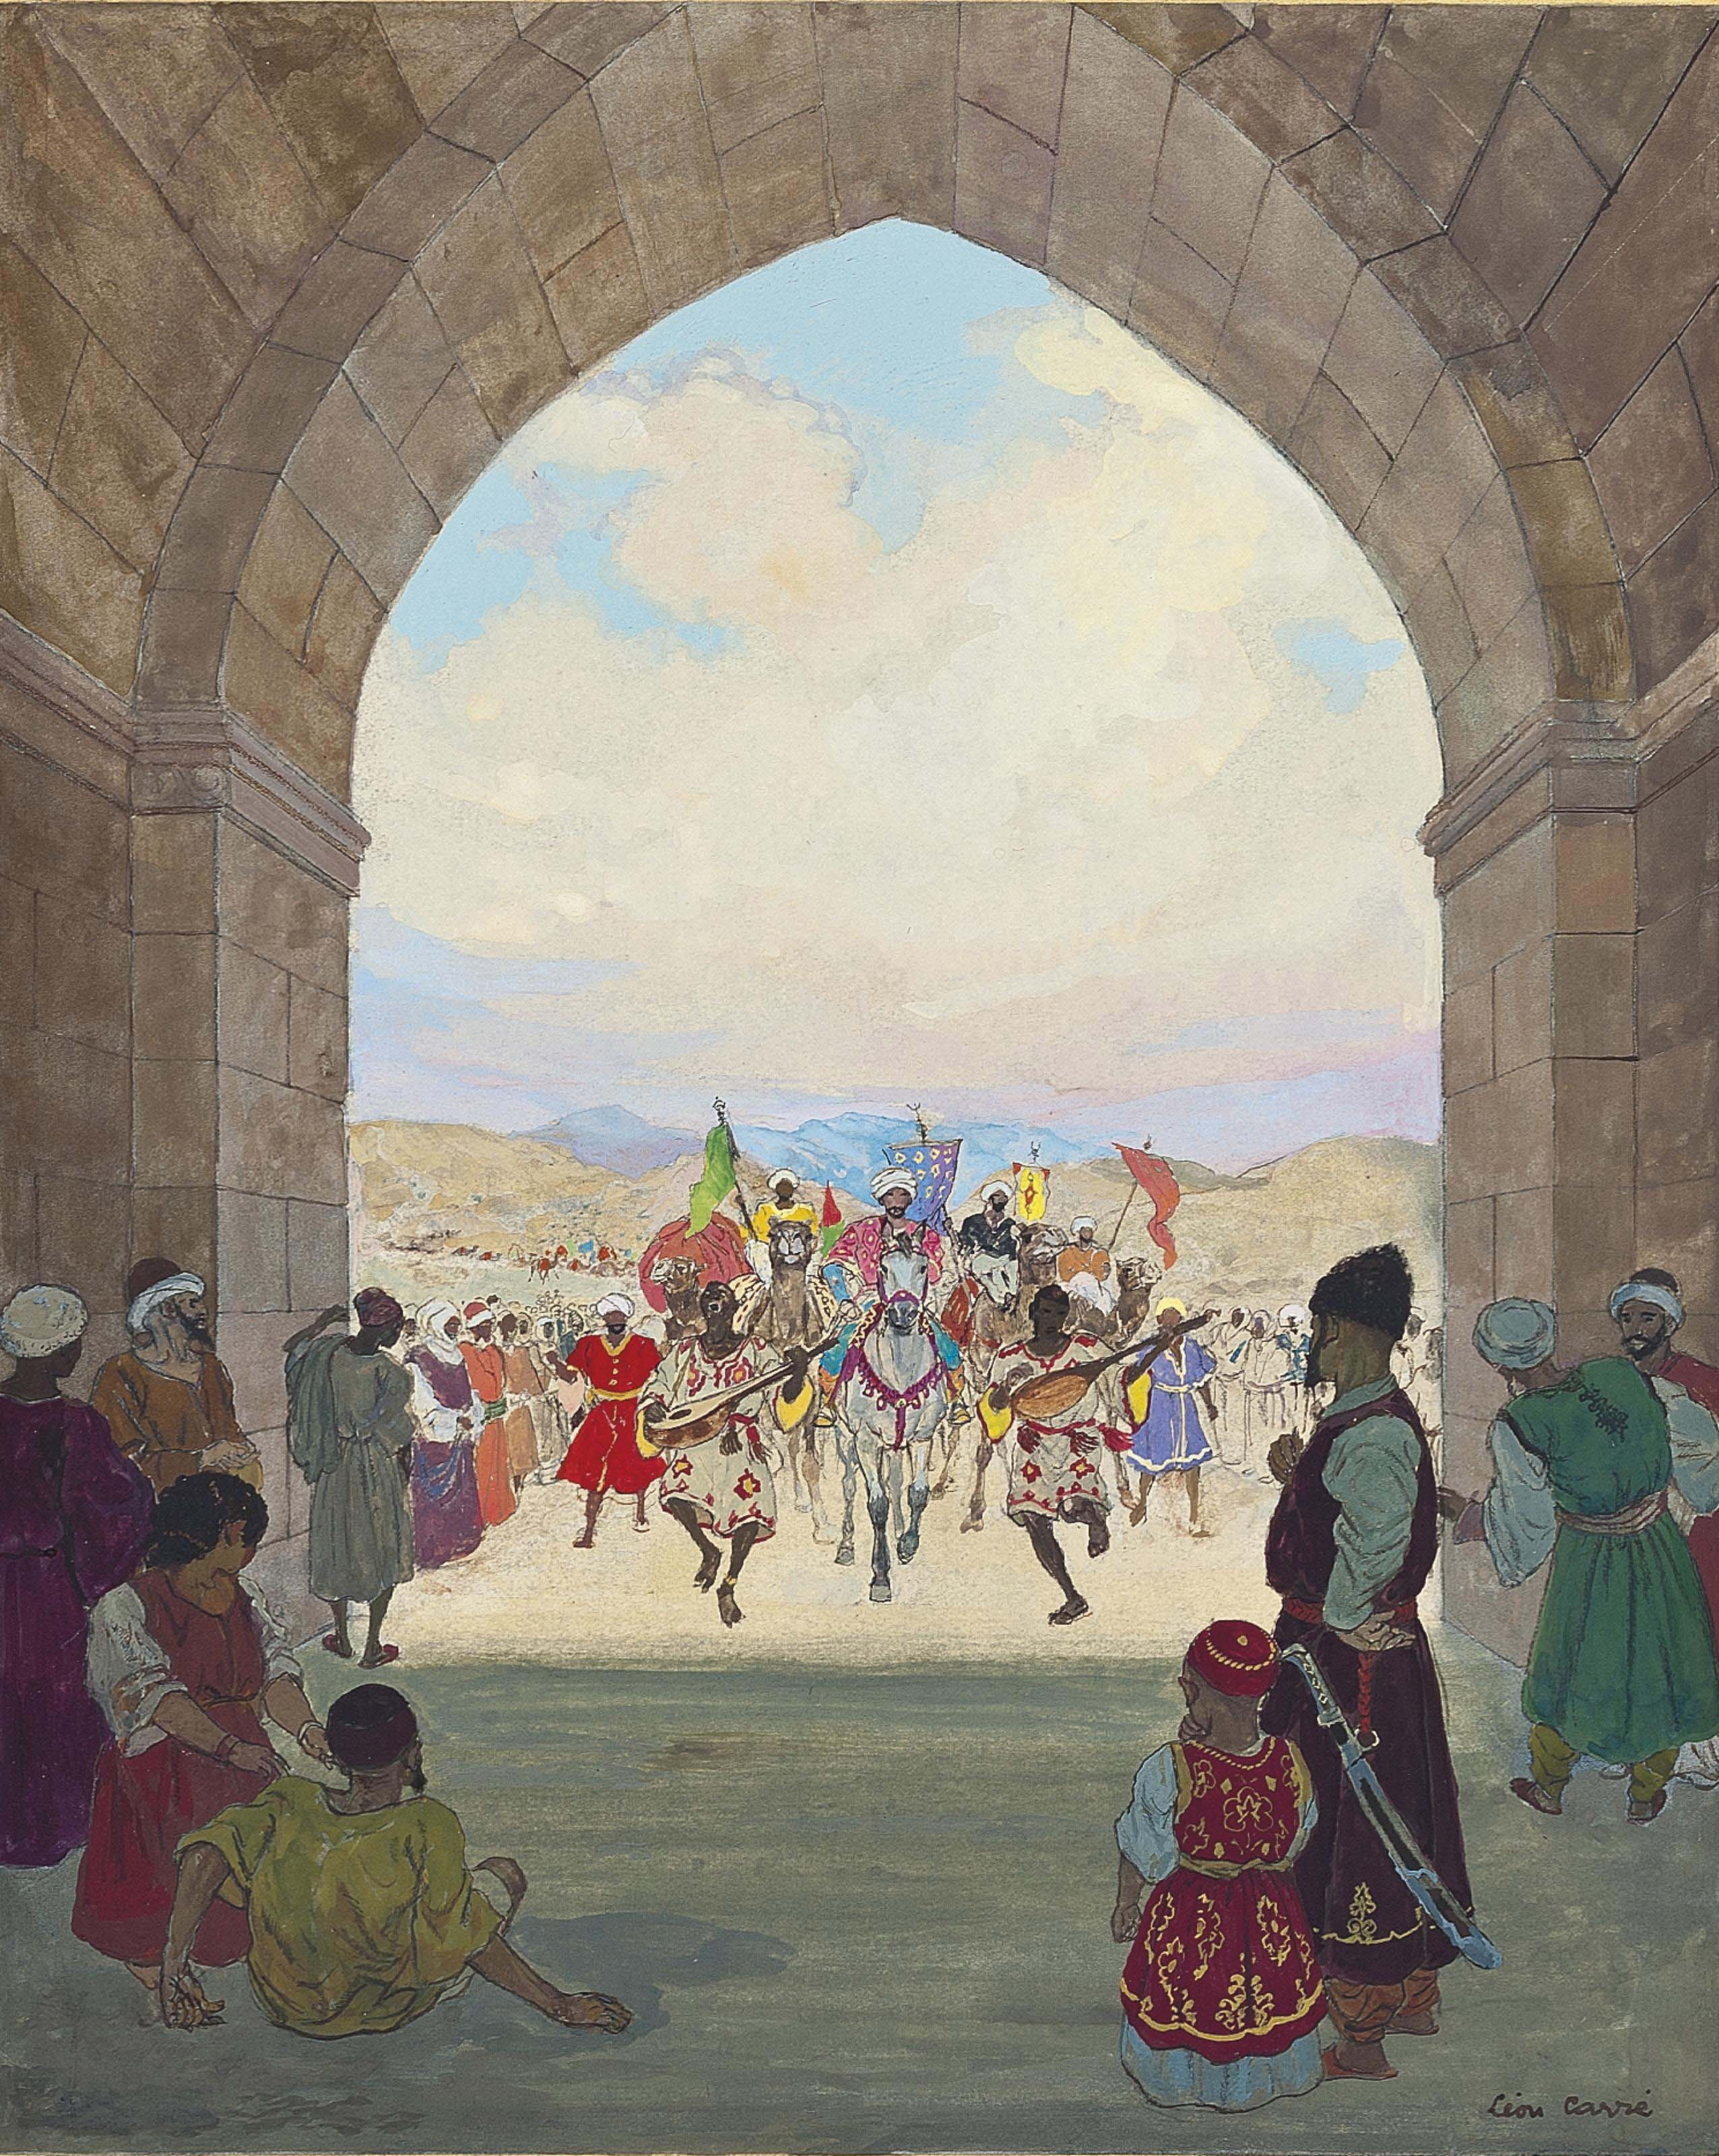
\includegraphics[height=\figsize]{illustrations/volume_8/T08, n0969 - Histoire du gateau échevelé au miel d'abeilles.jpg}
\end{figure}

\textit{\\
"...le cortège fit son entrée dans la ville. Et Mârouf chevauchait en tête, plus brillant mille fois que le roi, et magnifique et triomphant..."} \\
—T08, n0969 - Histoire du gateau échevelé au miel d'abeilles \\~\\
\textit{"...the escort, which had gone out to meet the caravan, returned to the city, and Maaruf pranced at its head, triumphant, magnificent, a thousand times more splendid than a king..."} \\
—V04, n0969 - The tale of the honey cake

\newpage

\section{n0973}
\textbf{\Large{Windows on the garden of history [The poet Duraid]}} \\

\begin{figure}[ht]
\centering
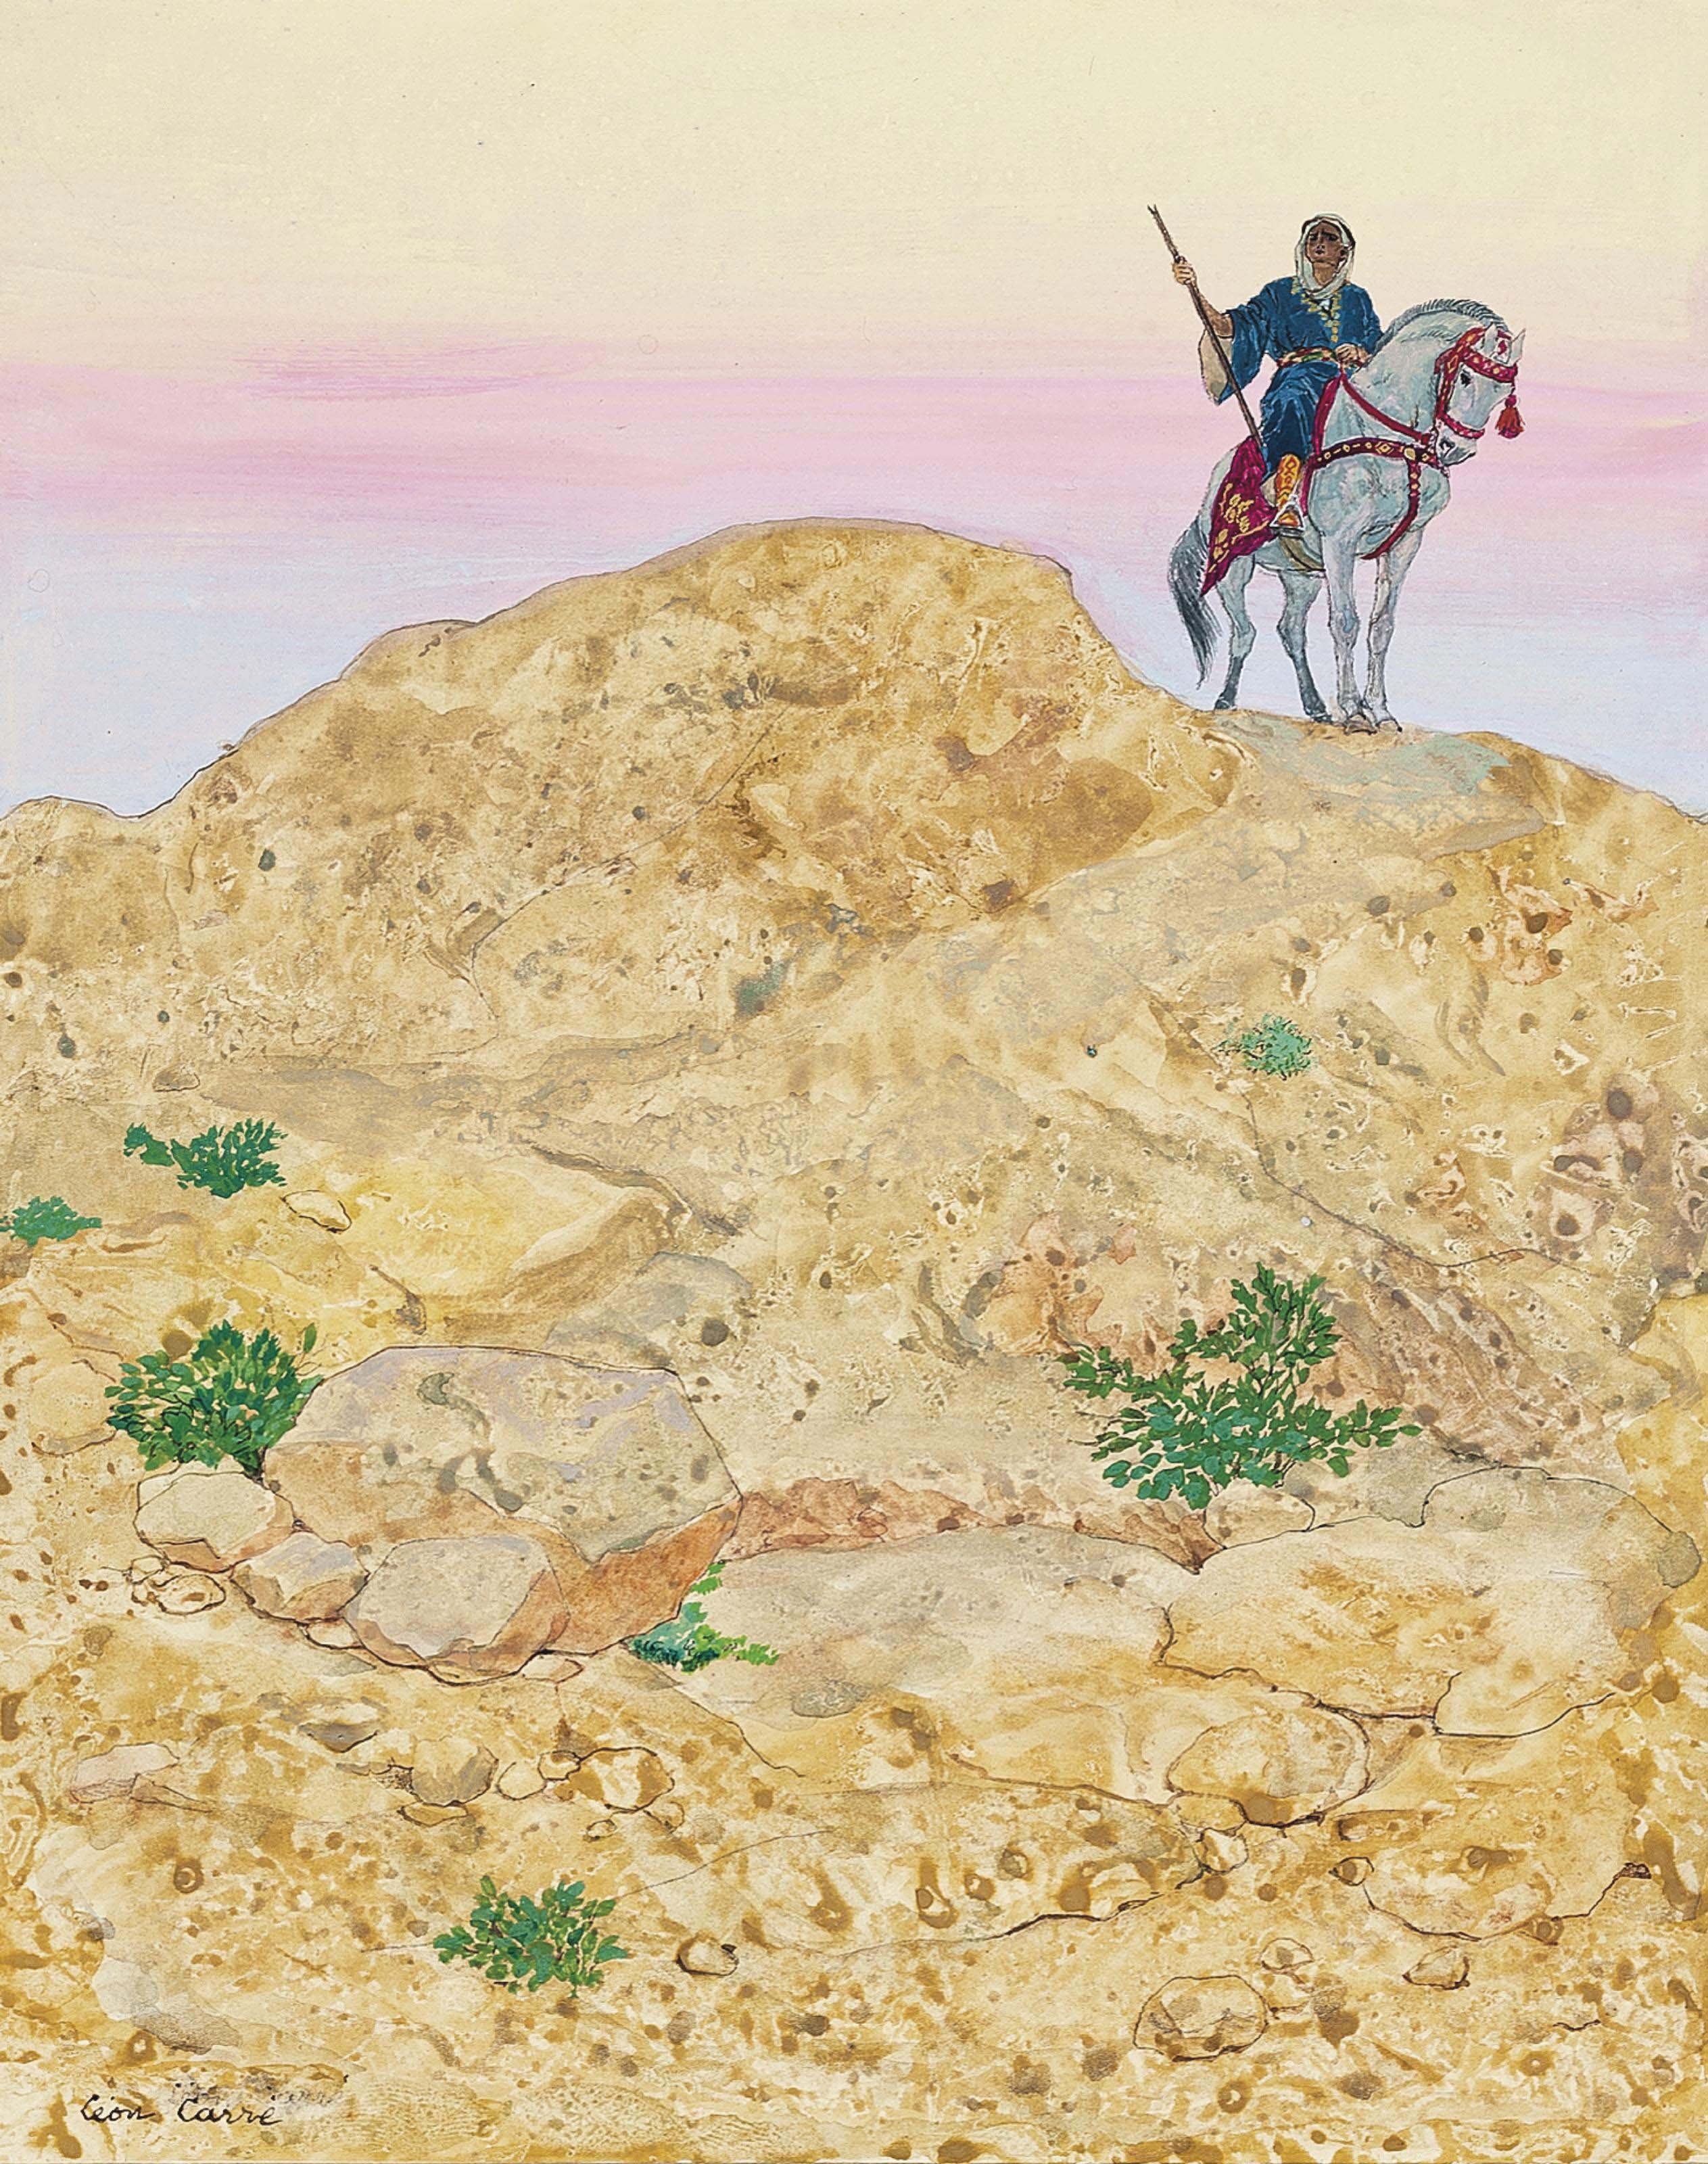
\includegraphics[height=\figsize]{illustrations/volume_8/T08, n0973 - Les lucarnes du savoir et de l'histoire [Le poète Doreïd].jpg}
\end{figure}

\textit{\\
"...Rabiah reconnut Doreïd, et regretta l’imprudence qu’il avait commise de ne s’être pas approprié la lance de son dernier agresseur. Toutefois il attendit Doreïd, droit sur sa selle, et le bois de sa lance brisée au poing."} \\
—T08, n0973 - Les lucarnes du savoir et de l'histoire [Le poète Doreïd] \\~\\
\textit{"Though the sheikh of the Banu Firas regretted that he had not armed himself from the corpse of his third adversary, yet he halted straight in the saddle, and faced Duraid with the broken wood of his lance firmly at tilt."} \\
—V04, n0973 - Windows on the garden of history [The poet Duraid]

\newpage

\section{n0977}
\textbf{\Large{Windows on the garden of history [Men in the judgment of their wives]}} \\

\begin{figure}[ht]
\centering
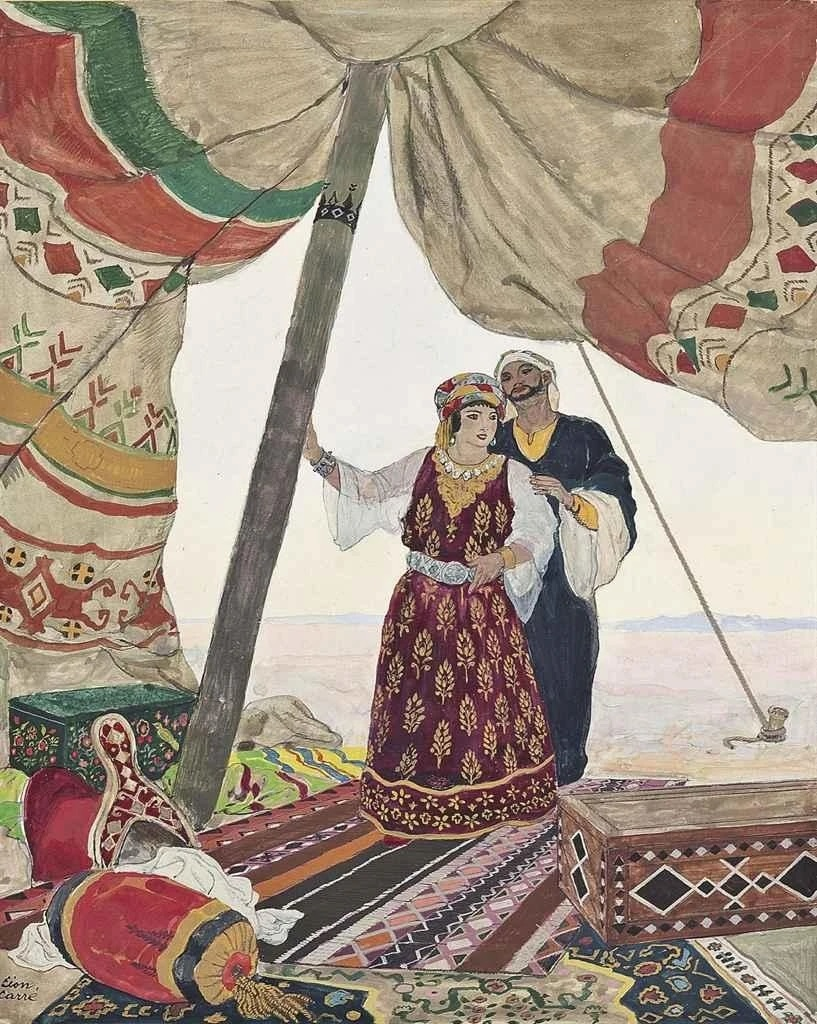
\includegraphics[height=\figsize]{illustrations/volume_8/T08, n0977 - Les lucarnes du savoir et de l'histoire [Les maries appréciés par leurs épouses].jpg}
\end{figure}

\textit{\\
"...moi, mon mari c’est Malik Abou-Zar, l’excellent Abou-Zar, connu de toutes nos tribus. Il m’a trouvée enfant d’une pauvre famille, dans la gêne et à l’étroit, et il m’a conduite dans sa tente aux belles couleurs..."} \\
—T08, n0977 - Les lucarnes du savoir et de l'histoire [Les maries appréciés par leurs épouses] \\~\\
\textit{"'My husband is Malik Abu Zar, that Abu Zar whom the tribes love. He found me the child of a poor house, he led me to his tent of colours..."} \\
—V04, n0977 - Windows on the garden of history [Men in the judgment of their wives]

\newpage

\section{n0982}
\textbf{\Large{Windows on the garden of history [The tale of the slave of destiny]}} \\

\begin{figure}[ht]
\centering
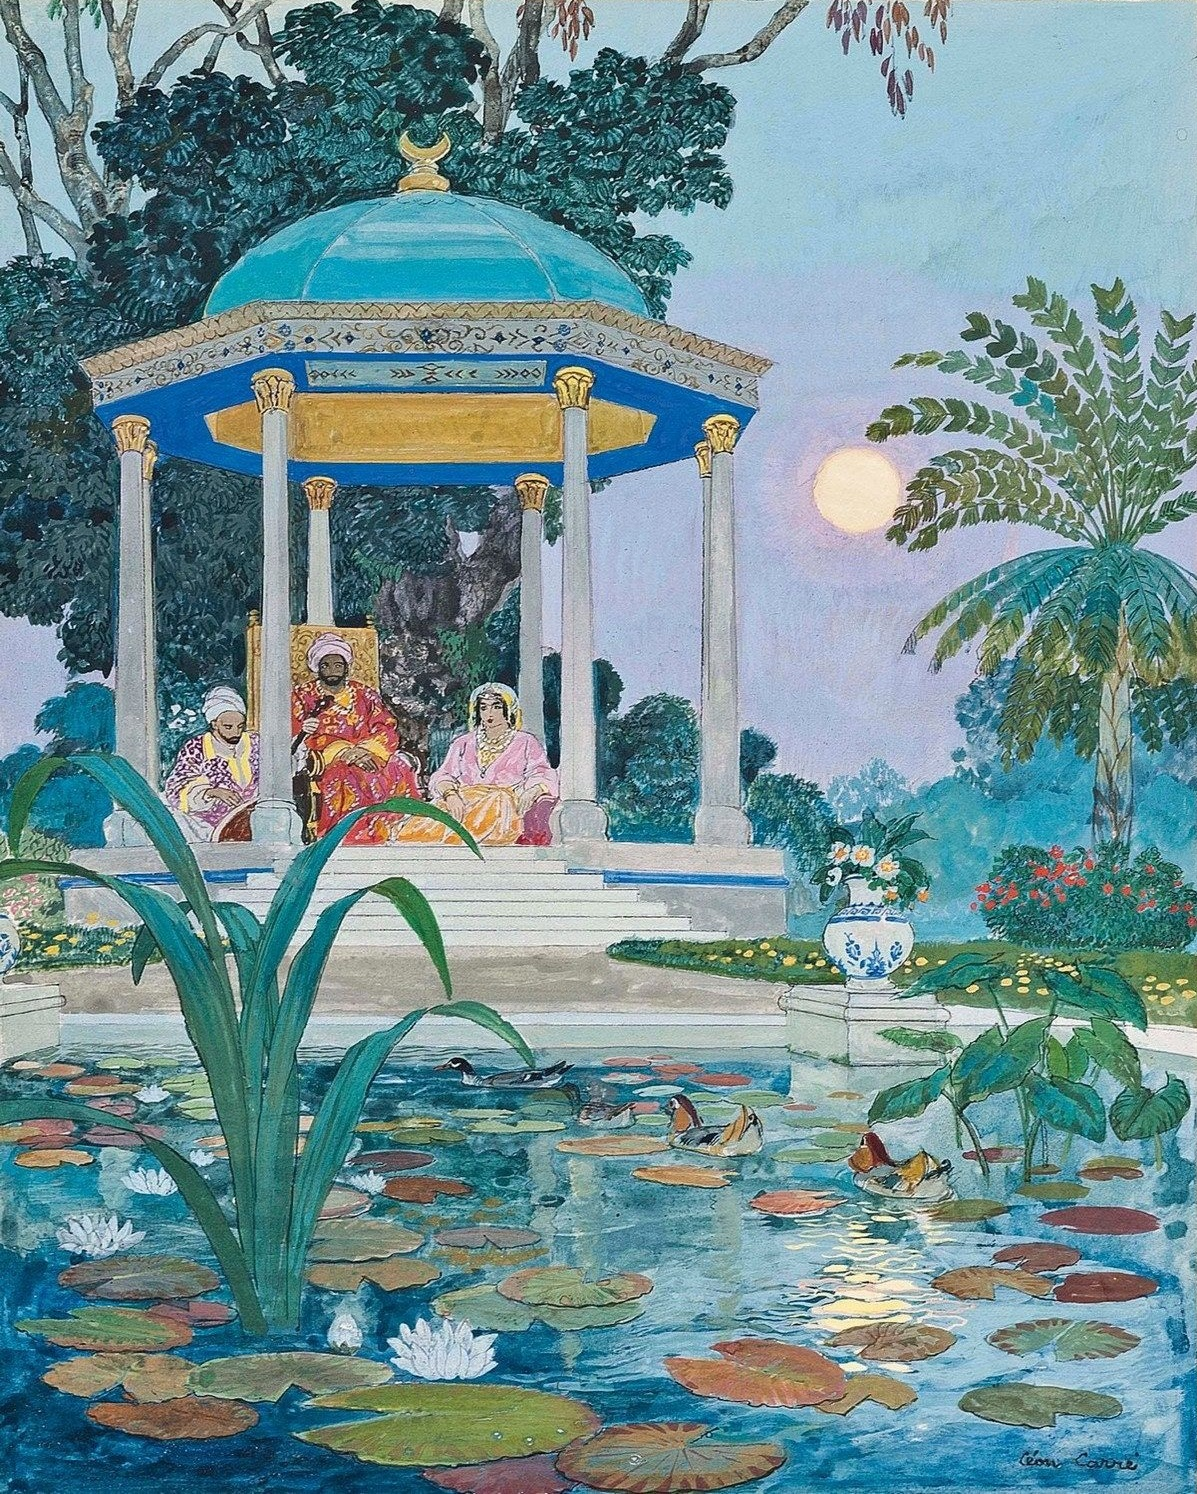
\includegraphics[height=\figsize]{illustrations/volume_8/T08, n0982 - Les lucarnes du savoir et de l'histoire [La favorite du destin].jpg}
\end{figure}

\textit{\\
"...Al-Hadi était un jour assis dans ses jardins, sous une riche coupole soutenue par huit colonnes, qui avait quatre entrées dont chacune regardait un des points du ciel."} \\
—T08, n0982 - Les lucarnes du savoir et de l'histoire [La favorite du destin] \\~\\
\textit{"One day al-Hadi sat in his garden, beneath a costly dome carried on eight columns and having four doors, each giving upon one of the cardinal points of the sky."} \\
—V04, n0982 - Windows on the garden of history [The tale of the slave of destiny]

\newpage

\section{n0998}
\textbf{\Large{The tender tale of prince Jasmine and princess Almond}} \\

\begin{figure}[ht]
\centering
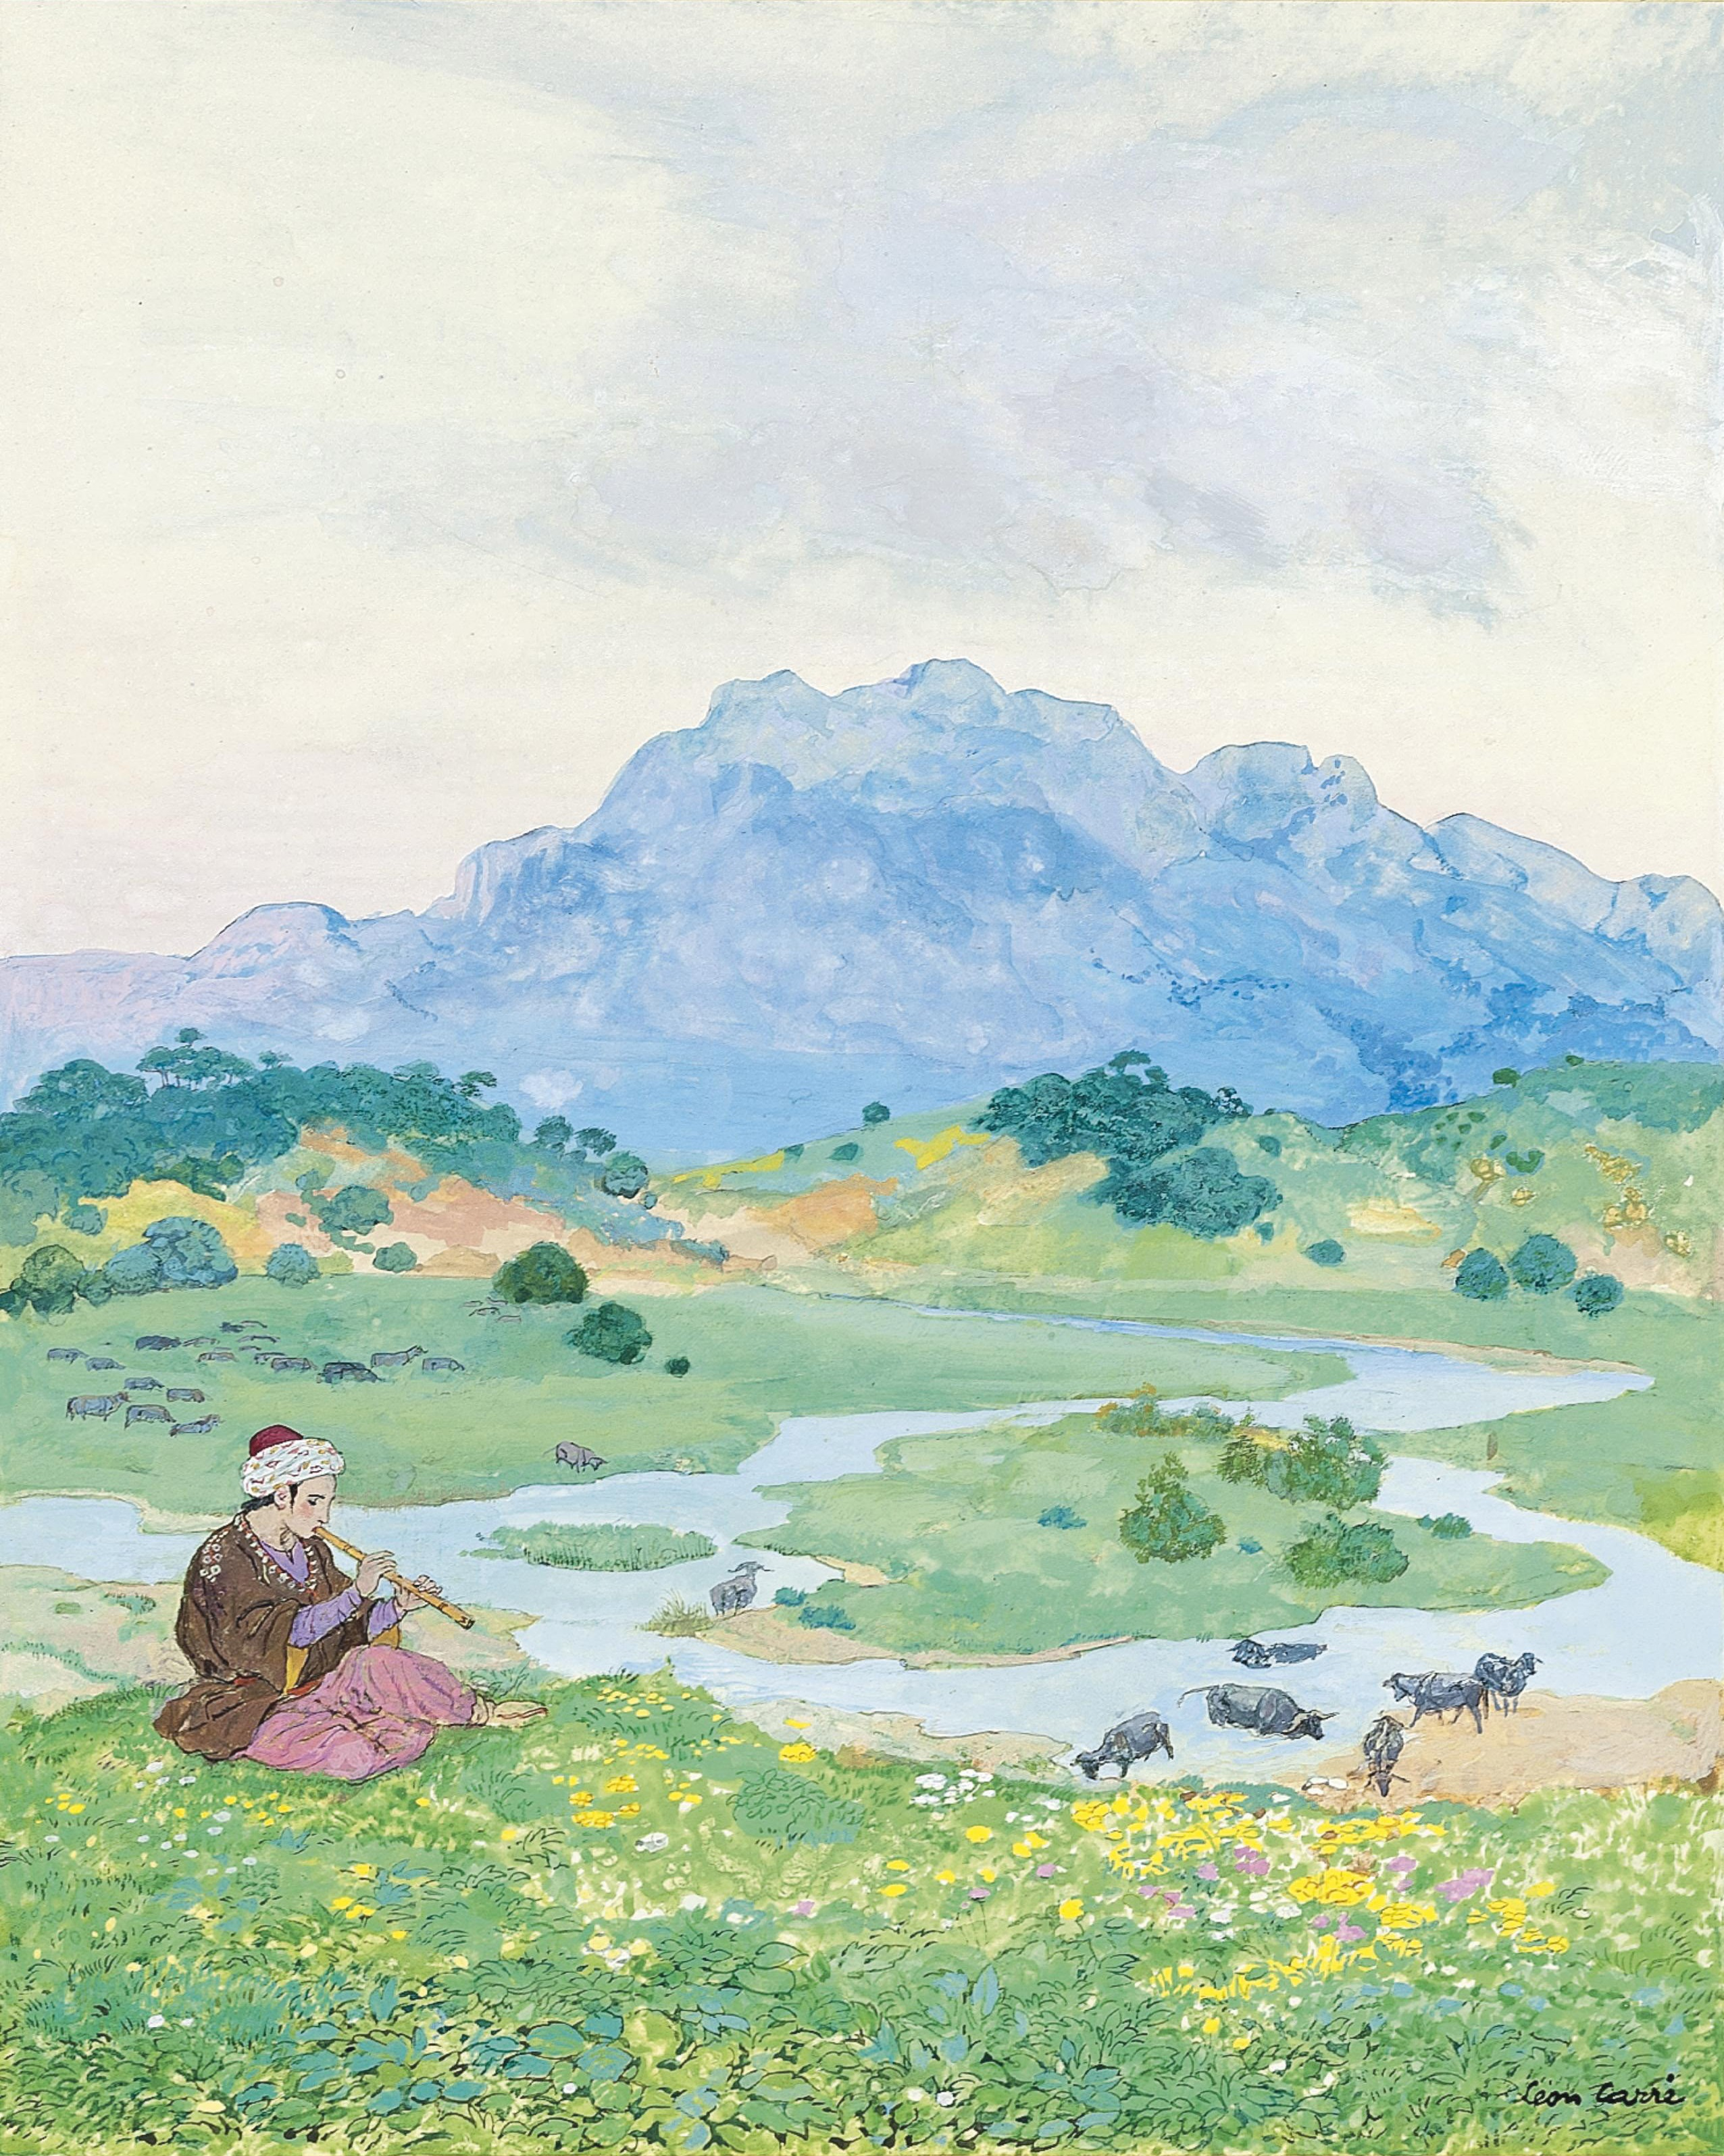
\includegraphics[height=\figsize]{illustrations/volume_8/T08, n0998 - Histoire du prince jasmin de la princesse amande.jpg}
\end{figure}

\textit{\\
"...sa demeure était dans les vastes solitudes et les pâturages. Et il était un jour assis à surveiller ses bêtes, en jouant de la flûte, quand il vit s’avancer de son côté un vénérable derviche..."} \\
—T08, n0998 - Histoire du prince jasmin de la princesse amande \\~\\
\textit{"As he sat one day in the lonely pasturage, watching his charges and playing upon the flute, a venerable darwish approached him..."} \\
—V04, n0998 - The tender tale of prince Jasmine and princess Almond

\newpage

\section{n1001}
\textbf{\Large{The tender tale of prince Jasmine and princess Almond}} \\

\begin{figure}[ht]
\centering
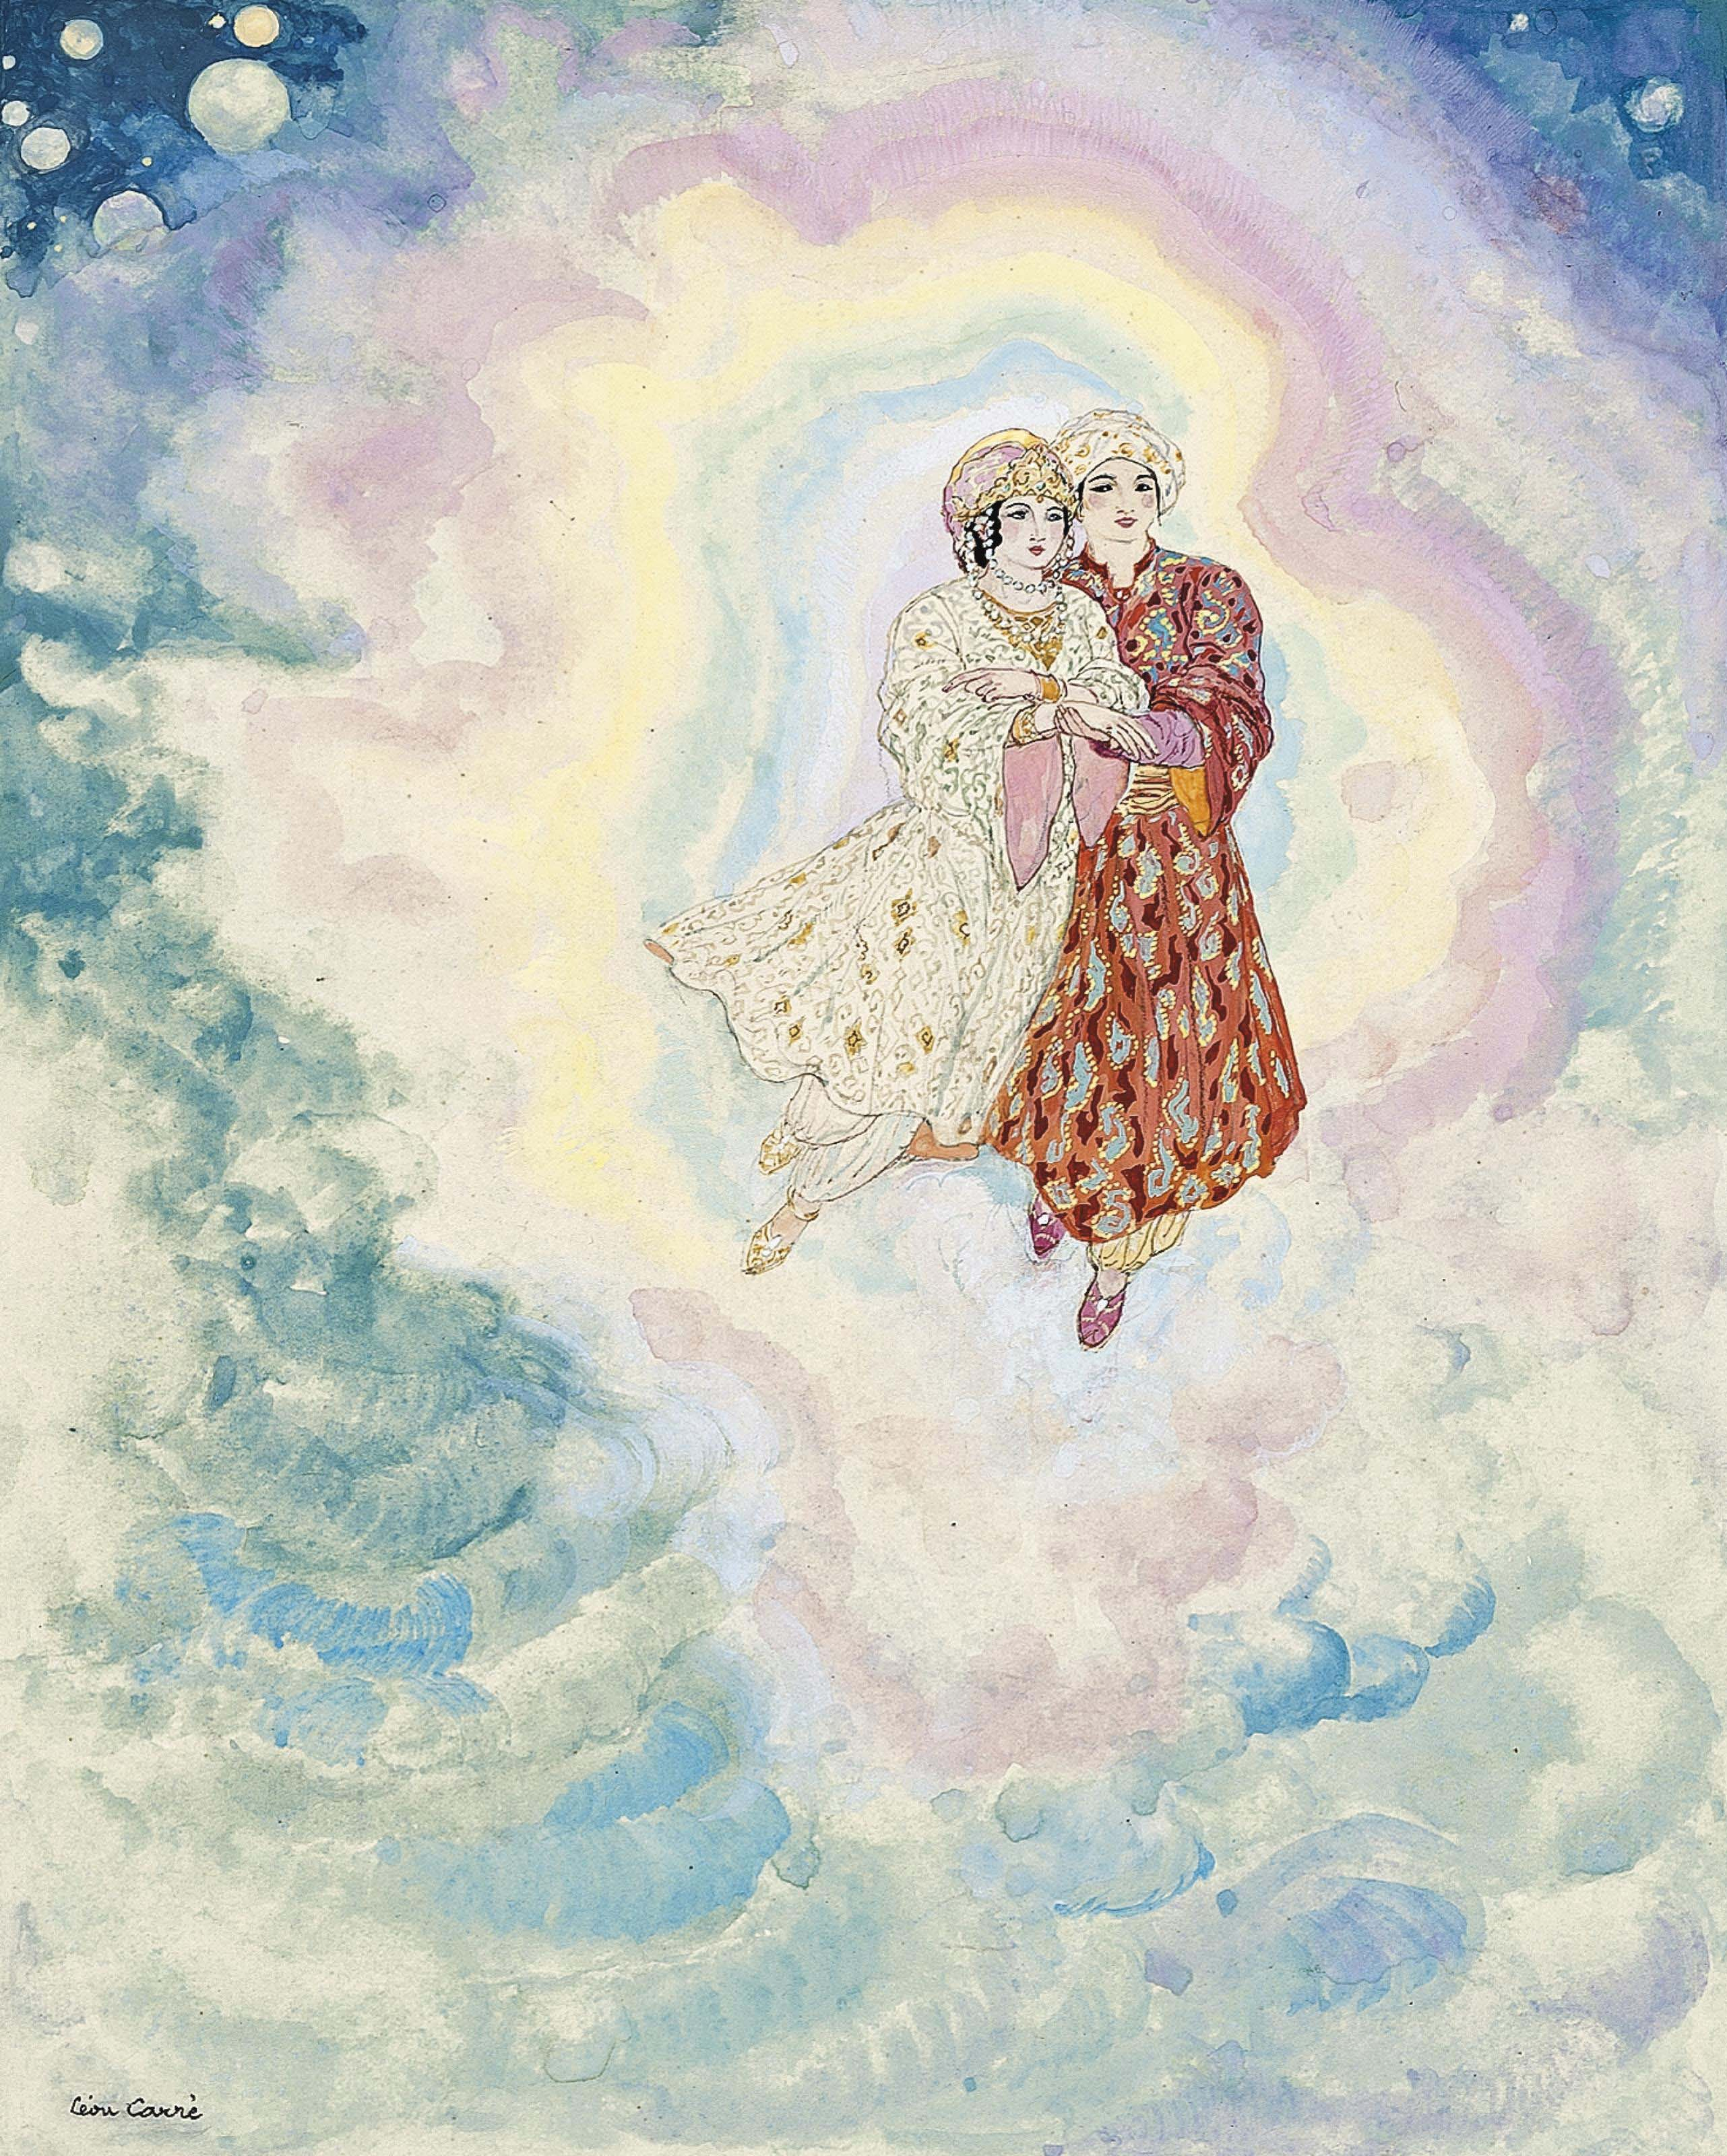
\includegraphics[height=\figsize]{illustrations/volume_8/T08, n1001 - Histoire du prince jasmin de la princesse amande.jpg}
\end{figure}

\textit{\\
"...ces deux amants bénis se prirent par la main et, plus légers que le zéphyr rosé, ils disparurent et s’évanouirent comme le camphre."} \\
—T08, n1001 - Histoire du prince jasmin de la princesse amande \\~\\
\textit{"These two delightful children took hands and vanished, more lightly than the dew-wet breeze of morning."} \\
—V04, n1001 - The tender tale of prince Jasmine and princess Almond

\end{document}